\section{Background and Motivation}
\label{sec:motivation}

\subsection{Existing Solutions of Container Networking}

P1: [Details and related work for existing container network solutions]There are two networking modes to inter-connect containers over multiple hosts:

\begin{itemize}
  \item Host mode: breaking the portability and independency
  \item Overlay mode: keeping the portability and independency
  \begin{itemize}
  \item Docker native overlay
  \item Weave
  \item Caliber (Optional)
  \end{itemize}  
\end{itemize}

\begin{figure}[ht]
     \centering 
     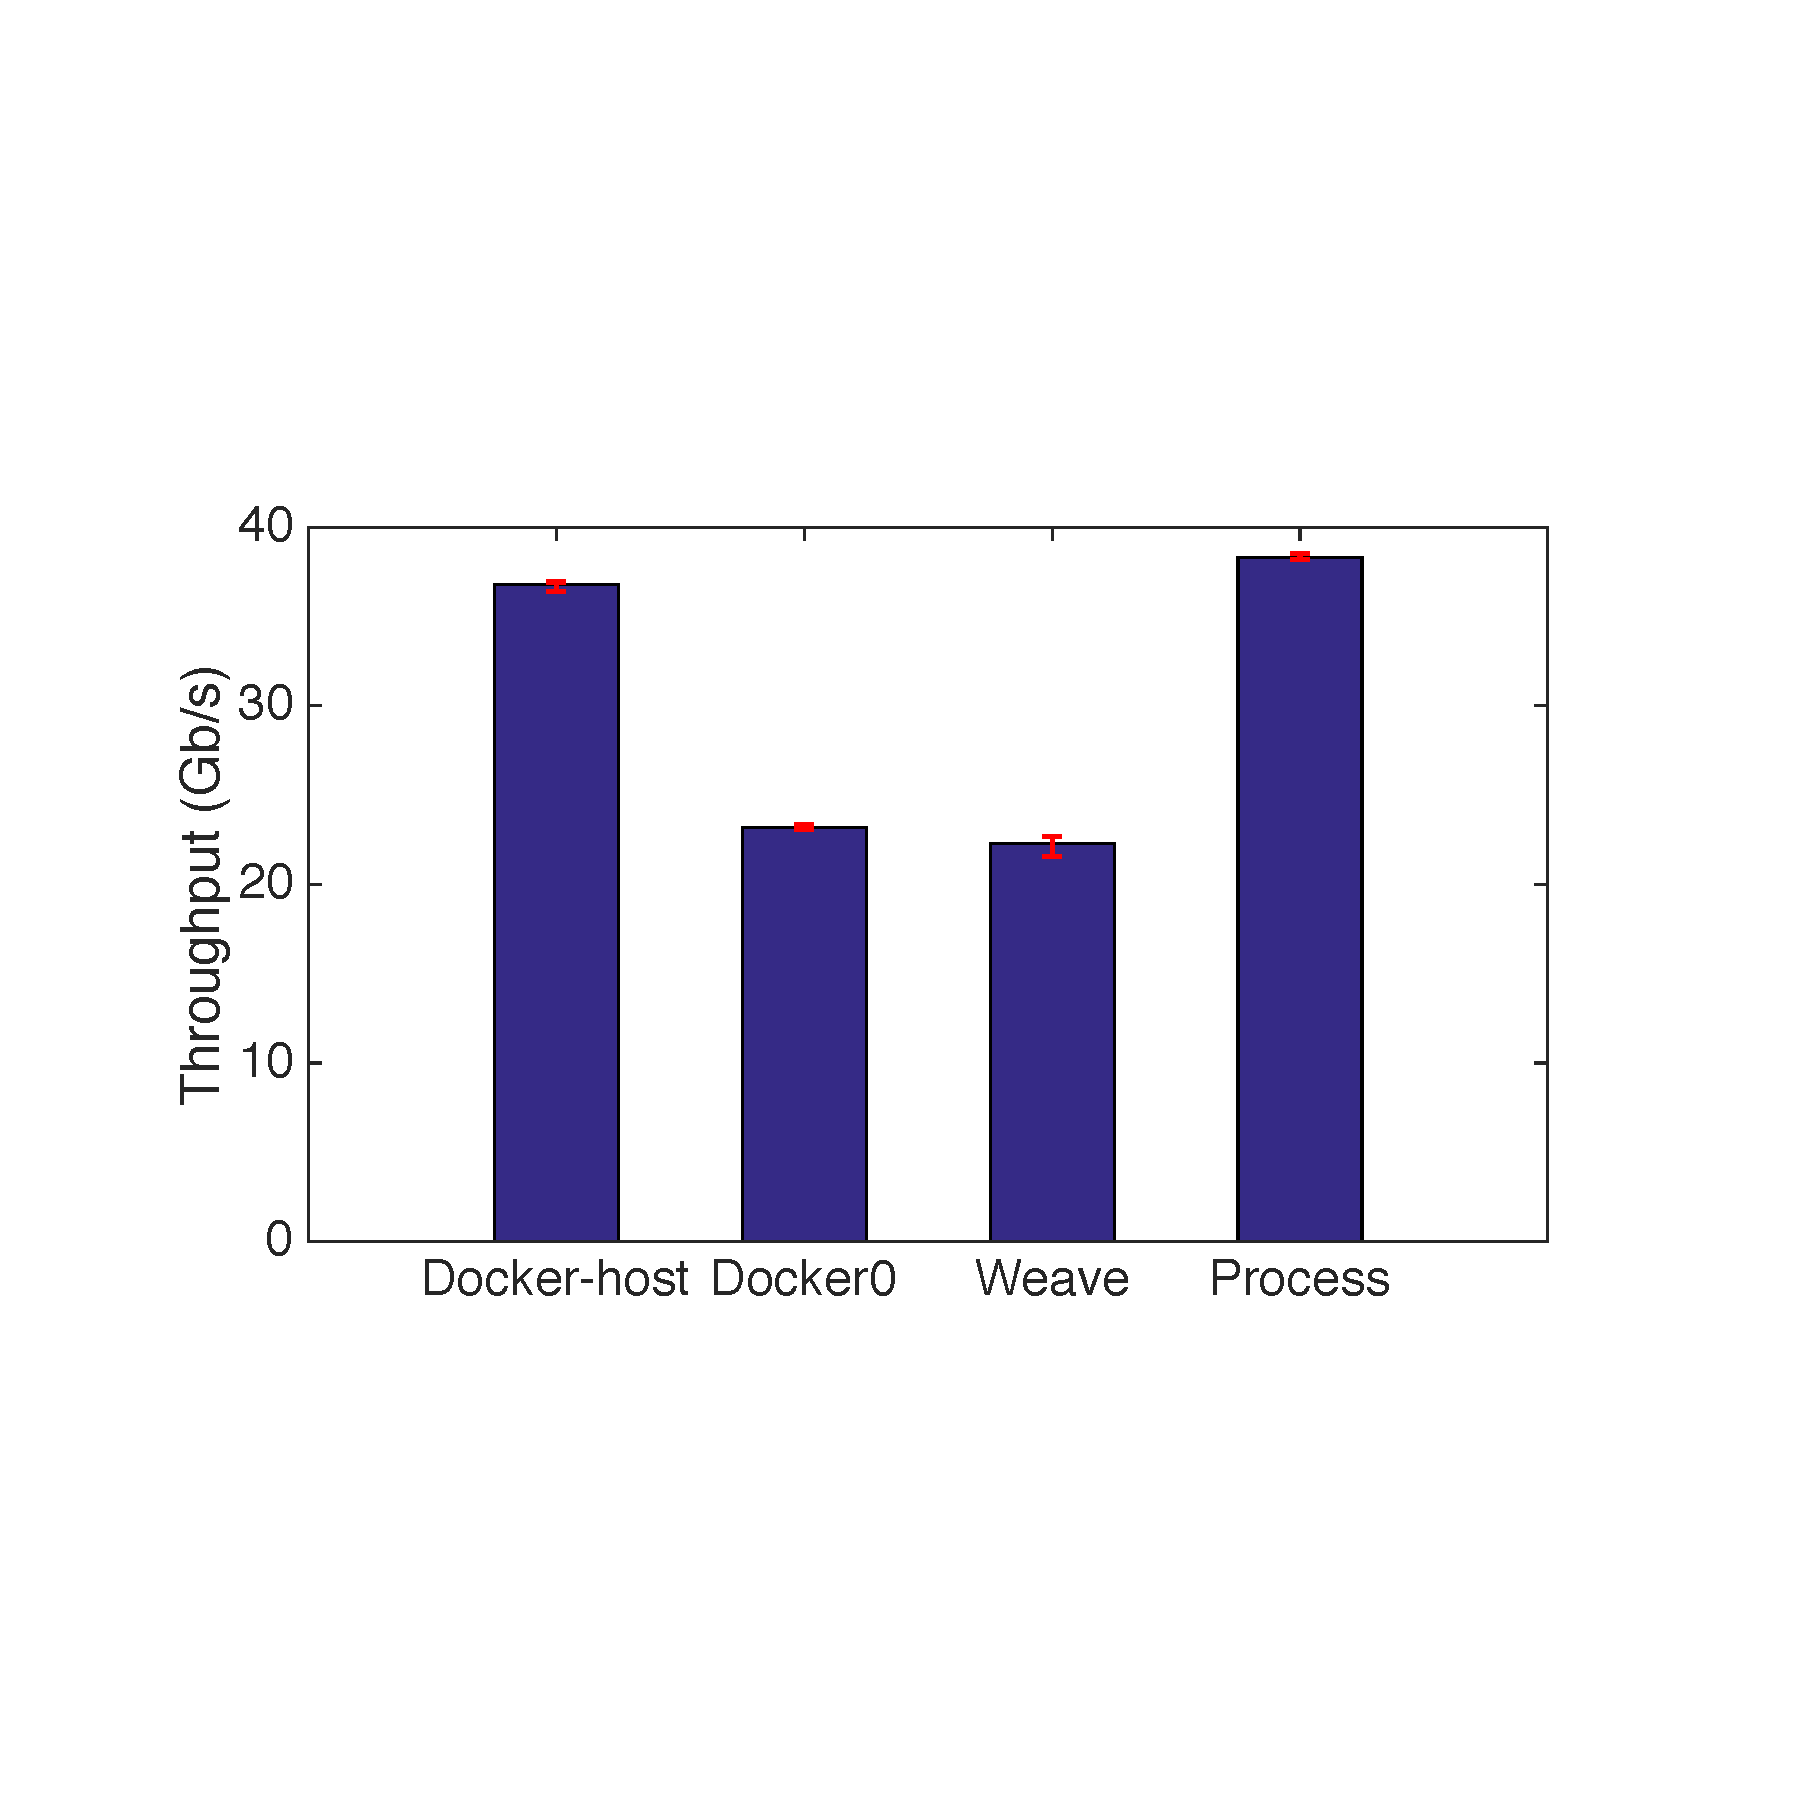
\includegraphics[width=0.35\textwidth]{figures/motivation/eval_exist_bw.pdf} 
     \label{fig:eval_exist_bw}
     \caption{The intra-host throughput of existing solutions. Docker-host is in host mode; Docker0 is in bridge mode; Weave is in overlay mode.} 
\end{figure} 

Conclusions:
\begin{itemize}
  \item The intra-host throughput of existing solutions are less than 40Gb/s.
  \item The throughput of two containers with host mode is close to the throughput of processes.
\end{itemize}

\subsection{Opportunities to build a better container networks}
P1: [Comparing container networking with other solutions]: In Sec 1, we have already seen the poor performance and high overhead of current container networking solution. Given containers are essentially processes, there are multiple better ways for two containers to communicate with each other.

\begin{itemize}
  \item Shared memory
  \item RDMA
  \item DPDK (not sure whether we have time to do it)
\end{itemize}

\subsubsection{Intra-host communication}

Throughput:
     \begin{figure}[ht]
     \centering 
     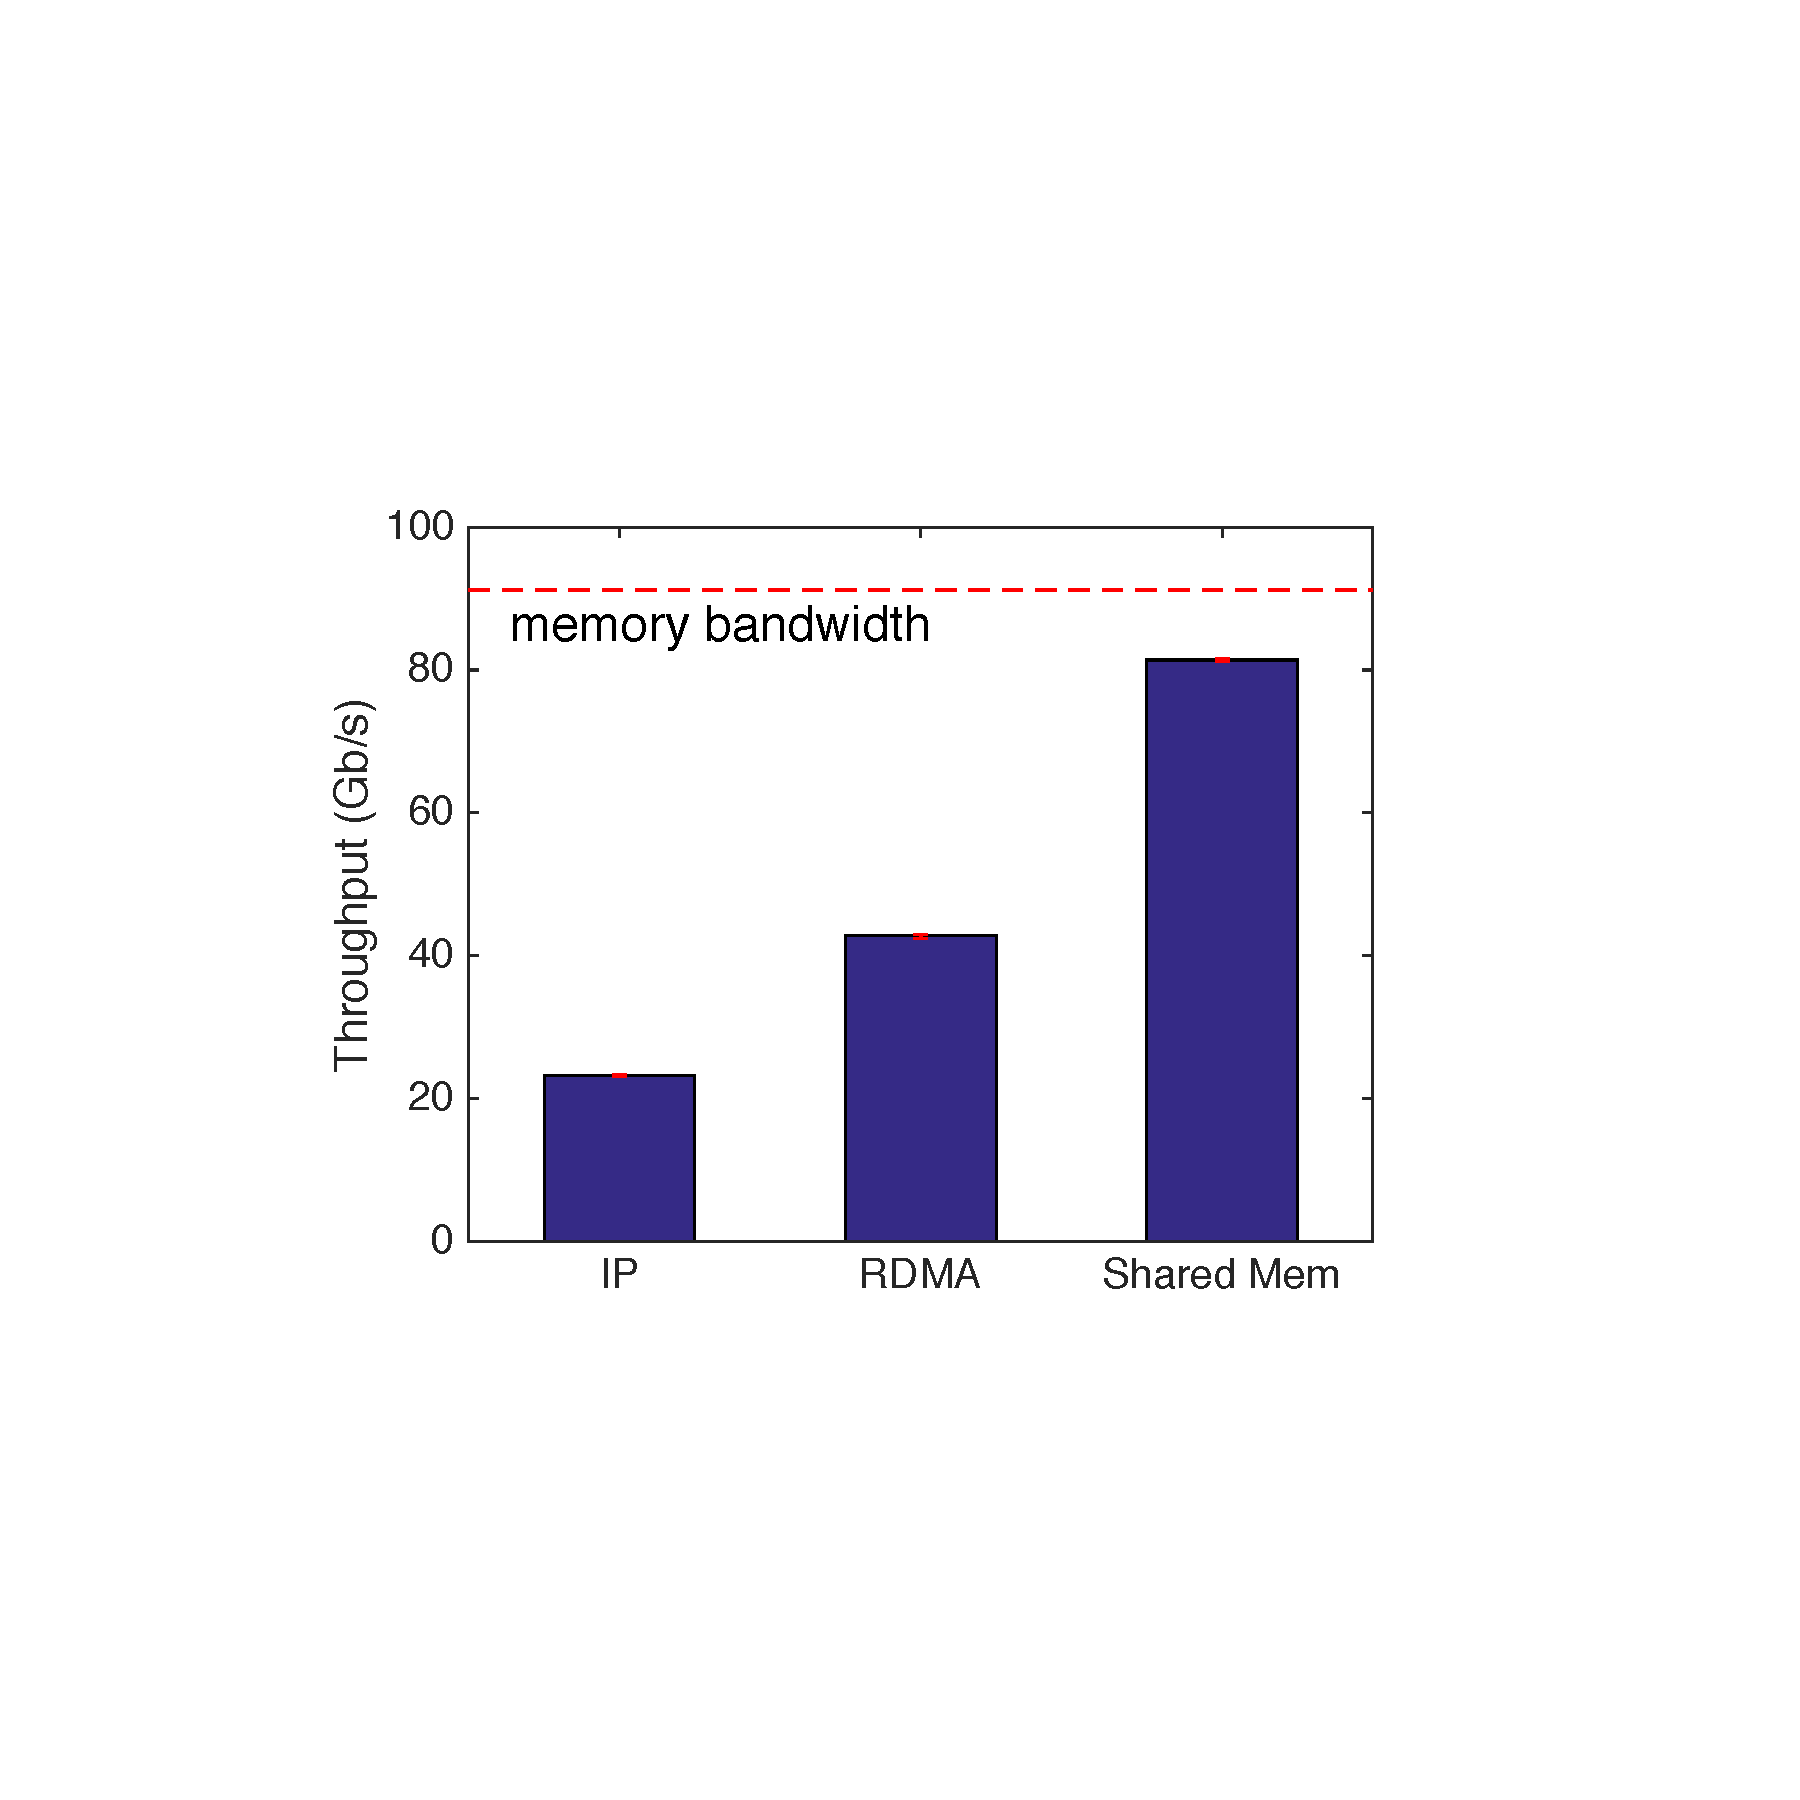
\includegraphics[width=0.32\textwidth]{figures/motivation/eval_baremetal_thr.pdf}      
     \label{fig:eval_baremetal_thr}
     \caption{} 
     \end{figure}

Latency:    
     \begin{figure}[ht]
     \centering 
     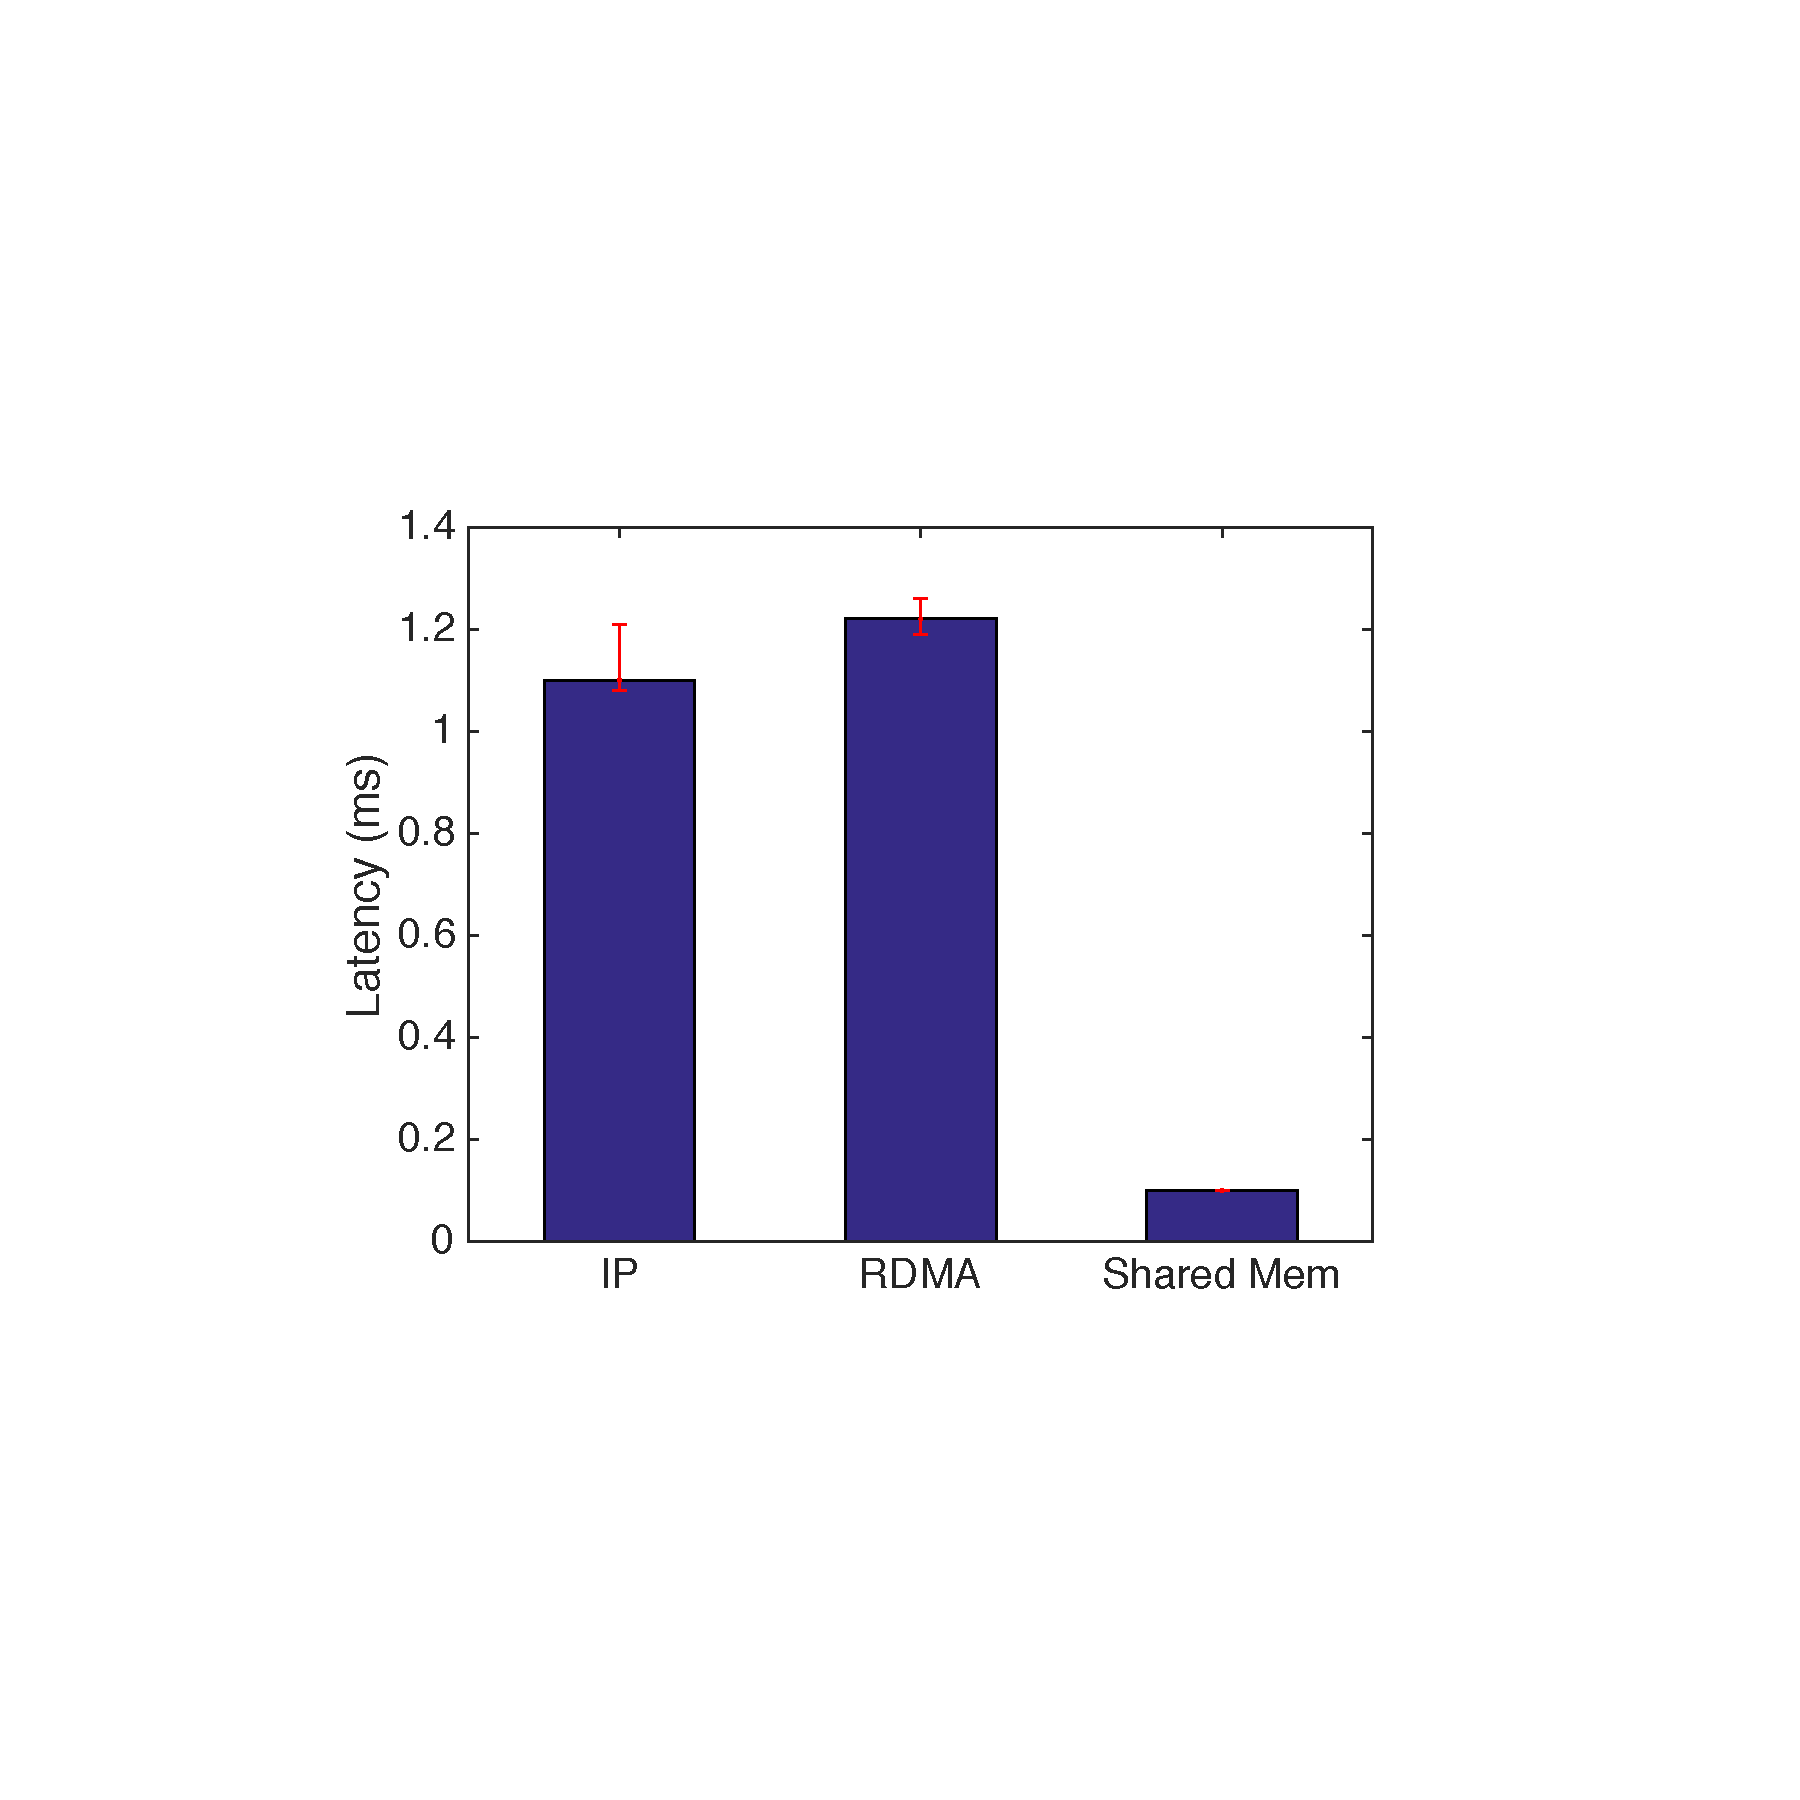
\includegraphics[width=0.32\textwidth]{figures/motivation/eval_baremetal_latency.pdf}      
     \label{fig:eval_baremetal_latency}
     \caption{} 
     \end{figure}

CPU usage:     
     \begin{figure}[ht]
     \centering 
     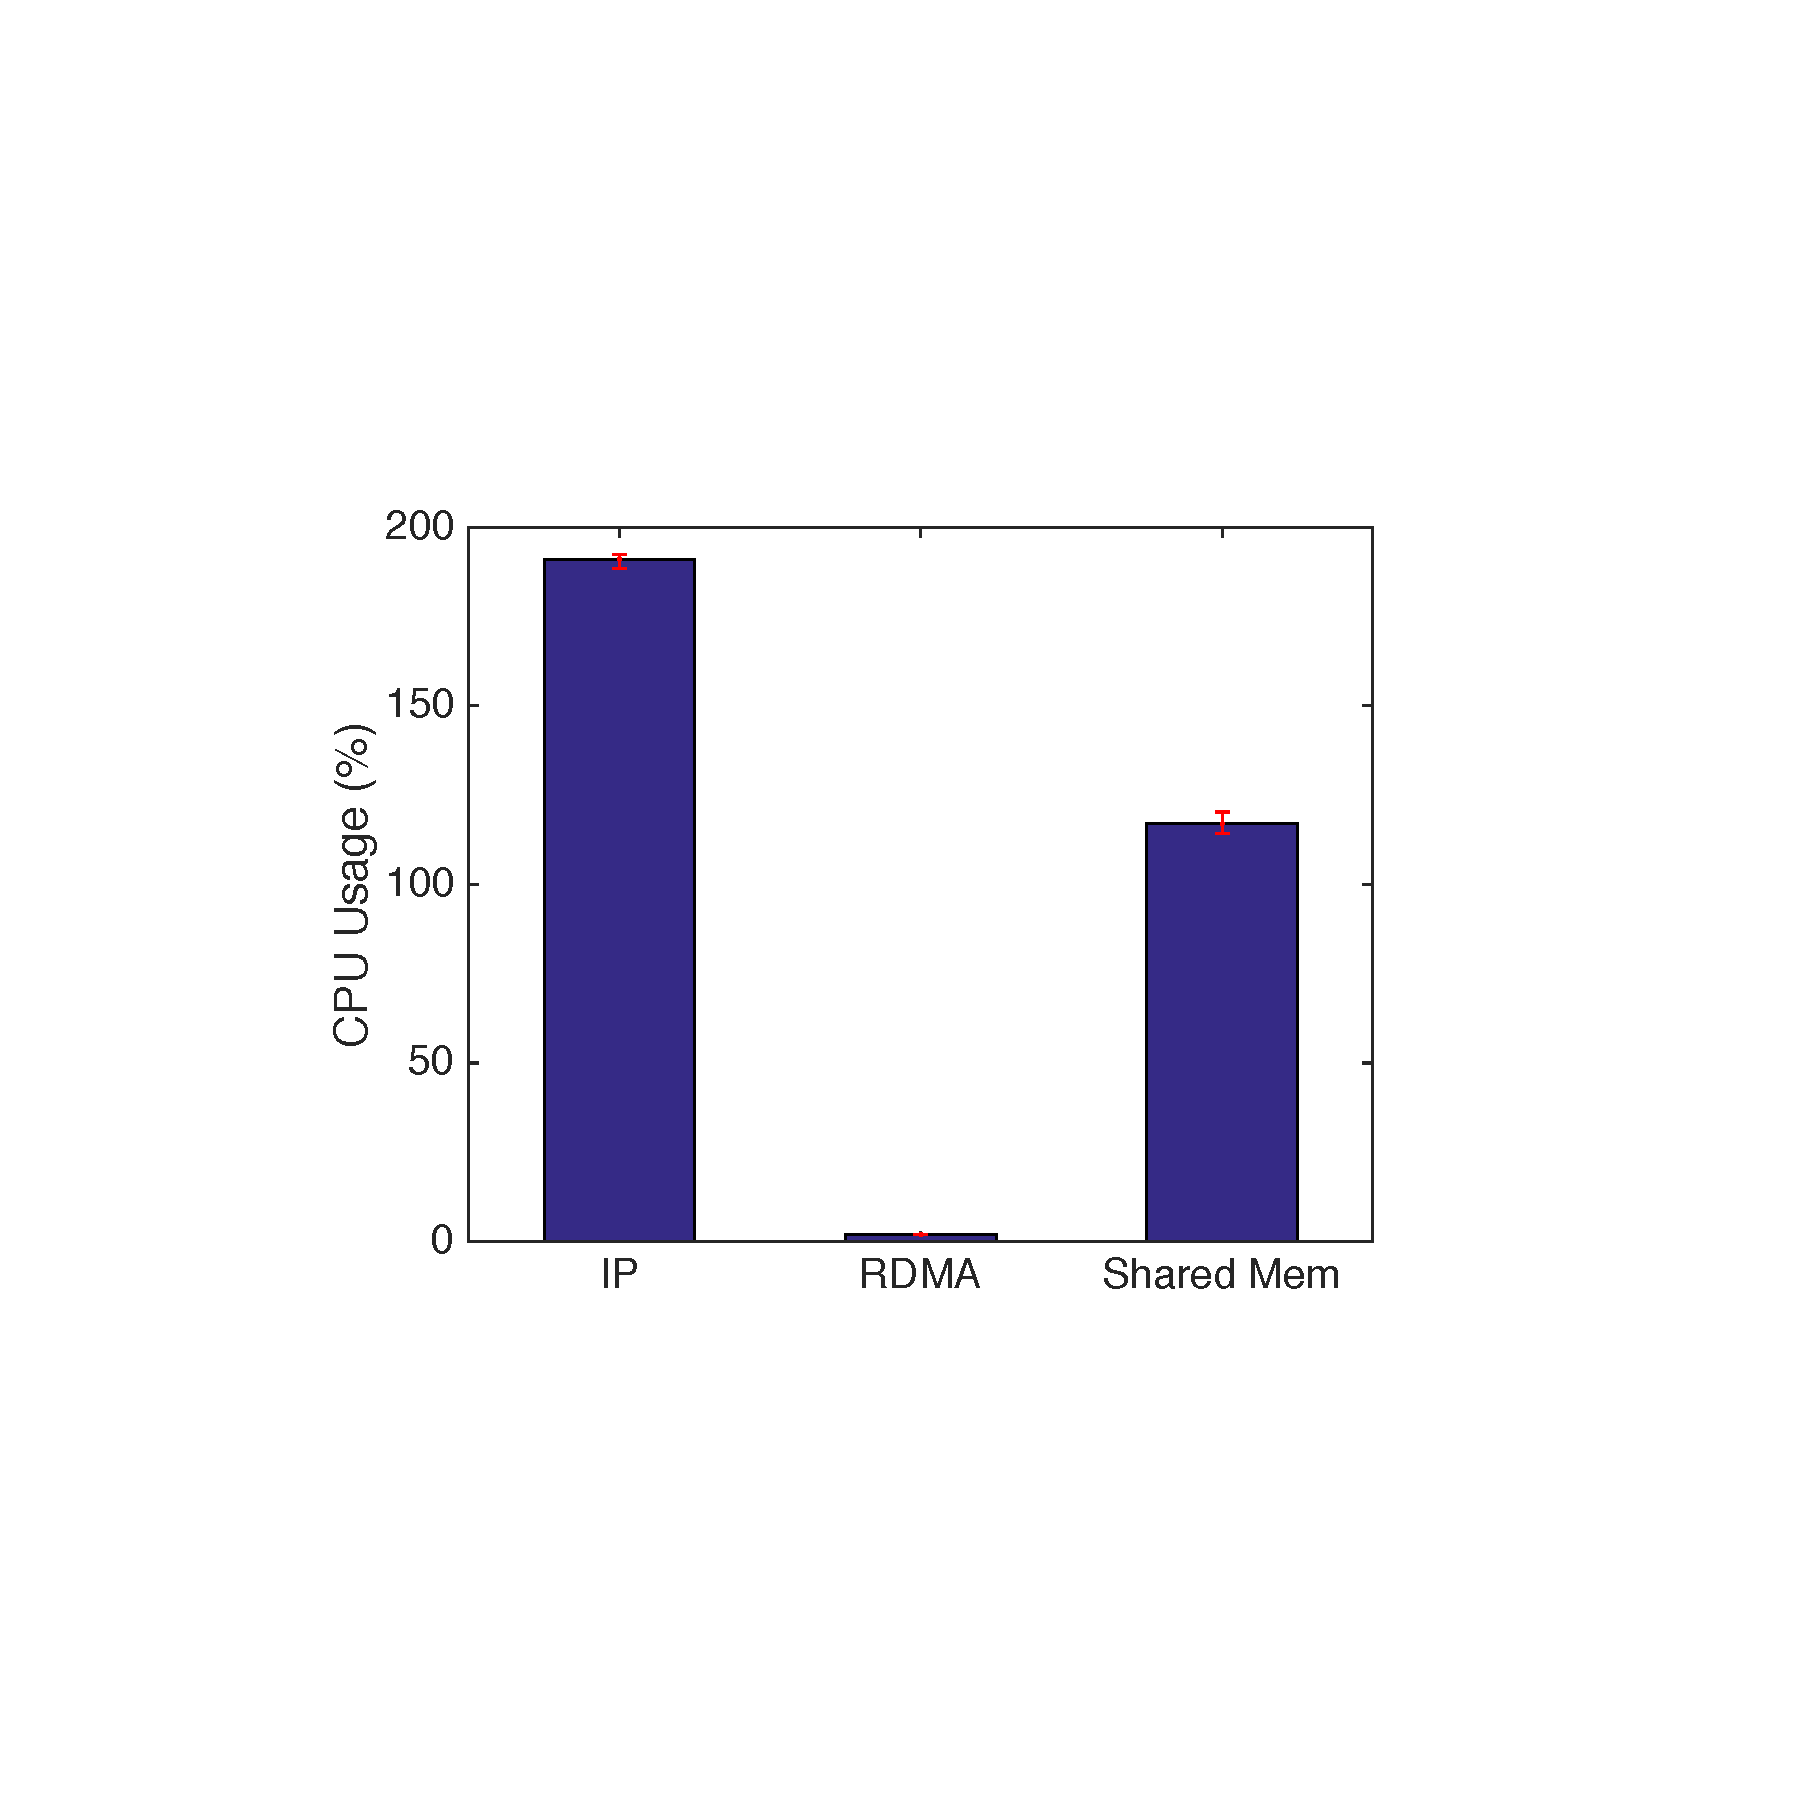
\includegraphics[width=0.32\textwidth]{figures/motivation/eval_baremetal_cpu.pdf}      
     \label{fig:eval_baremetal_cpu}
     \caption{} 
     \end{figure}
     
     \begin{figure}[ht]
     \centering 
     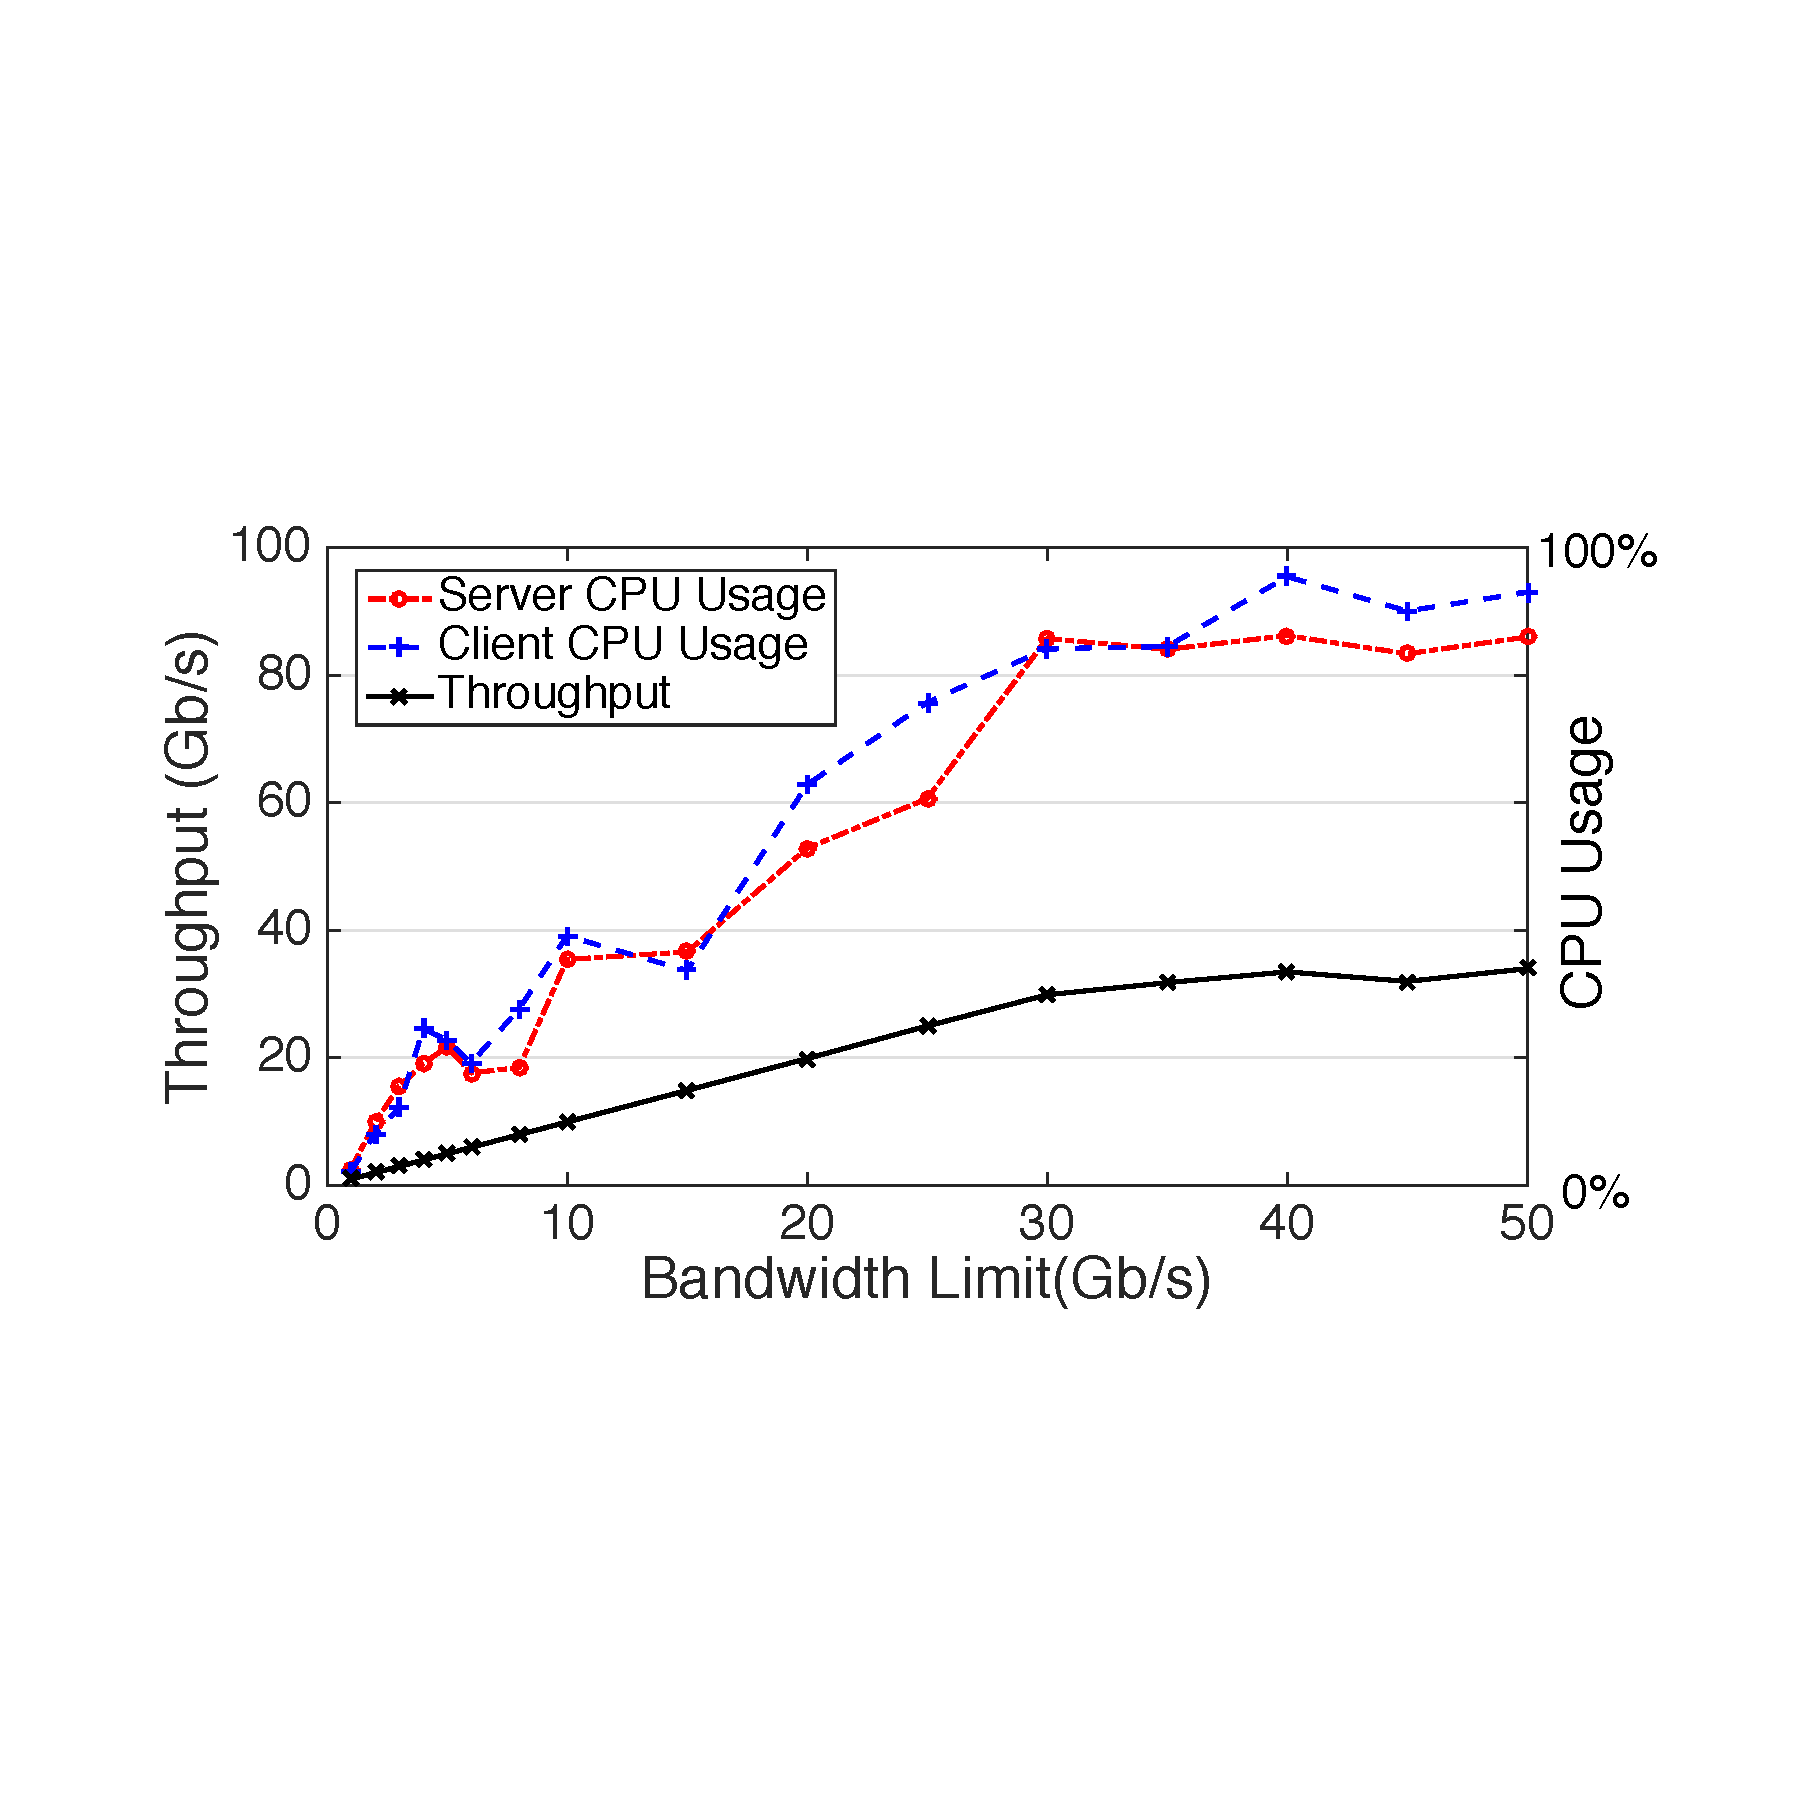
\includegraphics[width=0.4\textwidth]{figures/motivation/eval_bw_cpu.pdf}      
     \label{fig:eval_bw_cpu}
     \caption{} 
     \end{figure}
     
\begin{itemize}
  \item Communication via bridge mode only achieves 27Gb/s throughput, 1 ms latency but uses near to 200\% of cpu. (Host mode and overlay mode are similar.)
  \item RDMA only improves the throughput to 40Gb/s for containers on the same machine, the latency is still 1ms, though it has a low cpu usage.
  \item Shared memory can achieve near-to-memory-bandwidth throughput, lowest latency, but still burns some cpu. 
\end{itemize}


\subsubsection{Inter-host communication}



\subsection{Our Goals}
P1: [Goal] We want to build a container overlay networking solution which can guarantee the best network performance while keeping portability and independency for containers.

P2: [Specific requirements, challenges]
\begin{itemize}
  \item Smartly choosing network solutions (e.g. shared- memory, RDMA, DPDK, etc.) according to multiple factors.
  \item Making the network solution selection and switching be transparent to containers.
  \item IP assignments is independent to container's locations.
\end{itemize}

% comment 
\iffalse

* Figures:

* Throughput comparison (intra- and inter-host)

* CPU comparison

* Latency comparison

In this section, we present measurement results that demonstrates the network performance and resource overhead of different optional network channels. We focus on network throughput and latency when containers are located in the same or different hosts. 
We choose two kinds of hosts: physical machines and VMs in public clouds.

\subsection{Running environments of containers}

\begin{table} [t!]
\centering
\small
\begin{tabular}{ c || c | c | c | c }
  \hline
  Constraint & Case (a) & Case (b) & Case (c) & Case (d) \\ \hline \hline
  N/A & SharedMem & RDMA & SharedMem & RDMA \\ \hline
  w/o trust & TCP/IP & TCP/IP & TCP/IP & TCP/IP \\ \hline
  w/o RDMA NIC & SharedMem & TCP/IP & SharedMem & TCP/IP \\ \hline
\end{tabular}
\caption{\label{tab:best-network} The suggested network solution under different running environments in Figure~\ref{fig:deploy-cases} and constraints.}
\normalsize
\end{table}

Nowadays, a containerlized application is usually composed by multiple containers. For example, each master and slave node in Hadoop is an invividual container; A web service can include layers, such as load balancer, web server,
in-memory cache and backend database, and eacy layer can be a distributed 
system with multiple containerlized nodes. These containers are usually 
deployed into a multi-host server cluster, and the deployment is usually 
controlled by a cluster orchestrator, e.g. Mesos~\cite{?}. Working as a single 
application, the containers need to exchange data, and the network performance
has a huge impact on the overall application performance. 

Introduce the four representative cases of Figure~\ref{fig:deploy-cases}...

\subsection{The ineffiencies in container networking}

We measure the throughput and latency of TCP/IP, Shared-Mem and RDMA under cases
(a) (b) (c) and (d).

\harry{RDMA and Shared-Mem is missing under (c) and (d)}.

\para{The measurement setup}
(1) two bare metals: 40Gbps NICs.
(2) two VMs on top of the two bare metals.
(3) two VMs from Azure or EC2.

\subsection{Intra-host performance}
\subsubsection{throughput vs. latency vs. cpu usage}

\begin{figure*}[t]
     \centering 
     %\begin{subfigure}[t]{0.25\textwidth}
     \begin{subfigure}[t]
     \centering 
     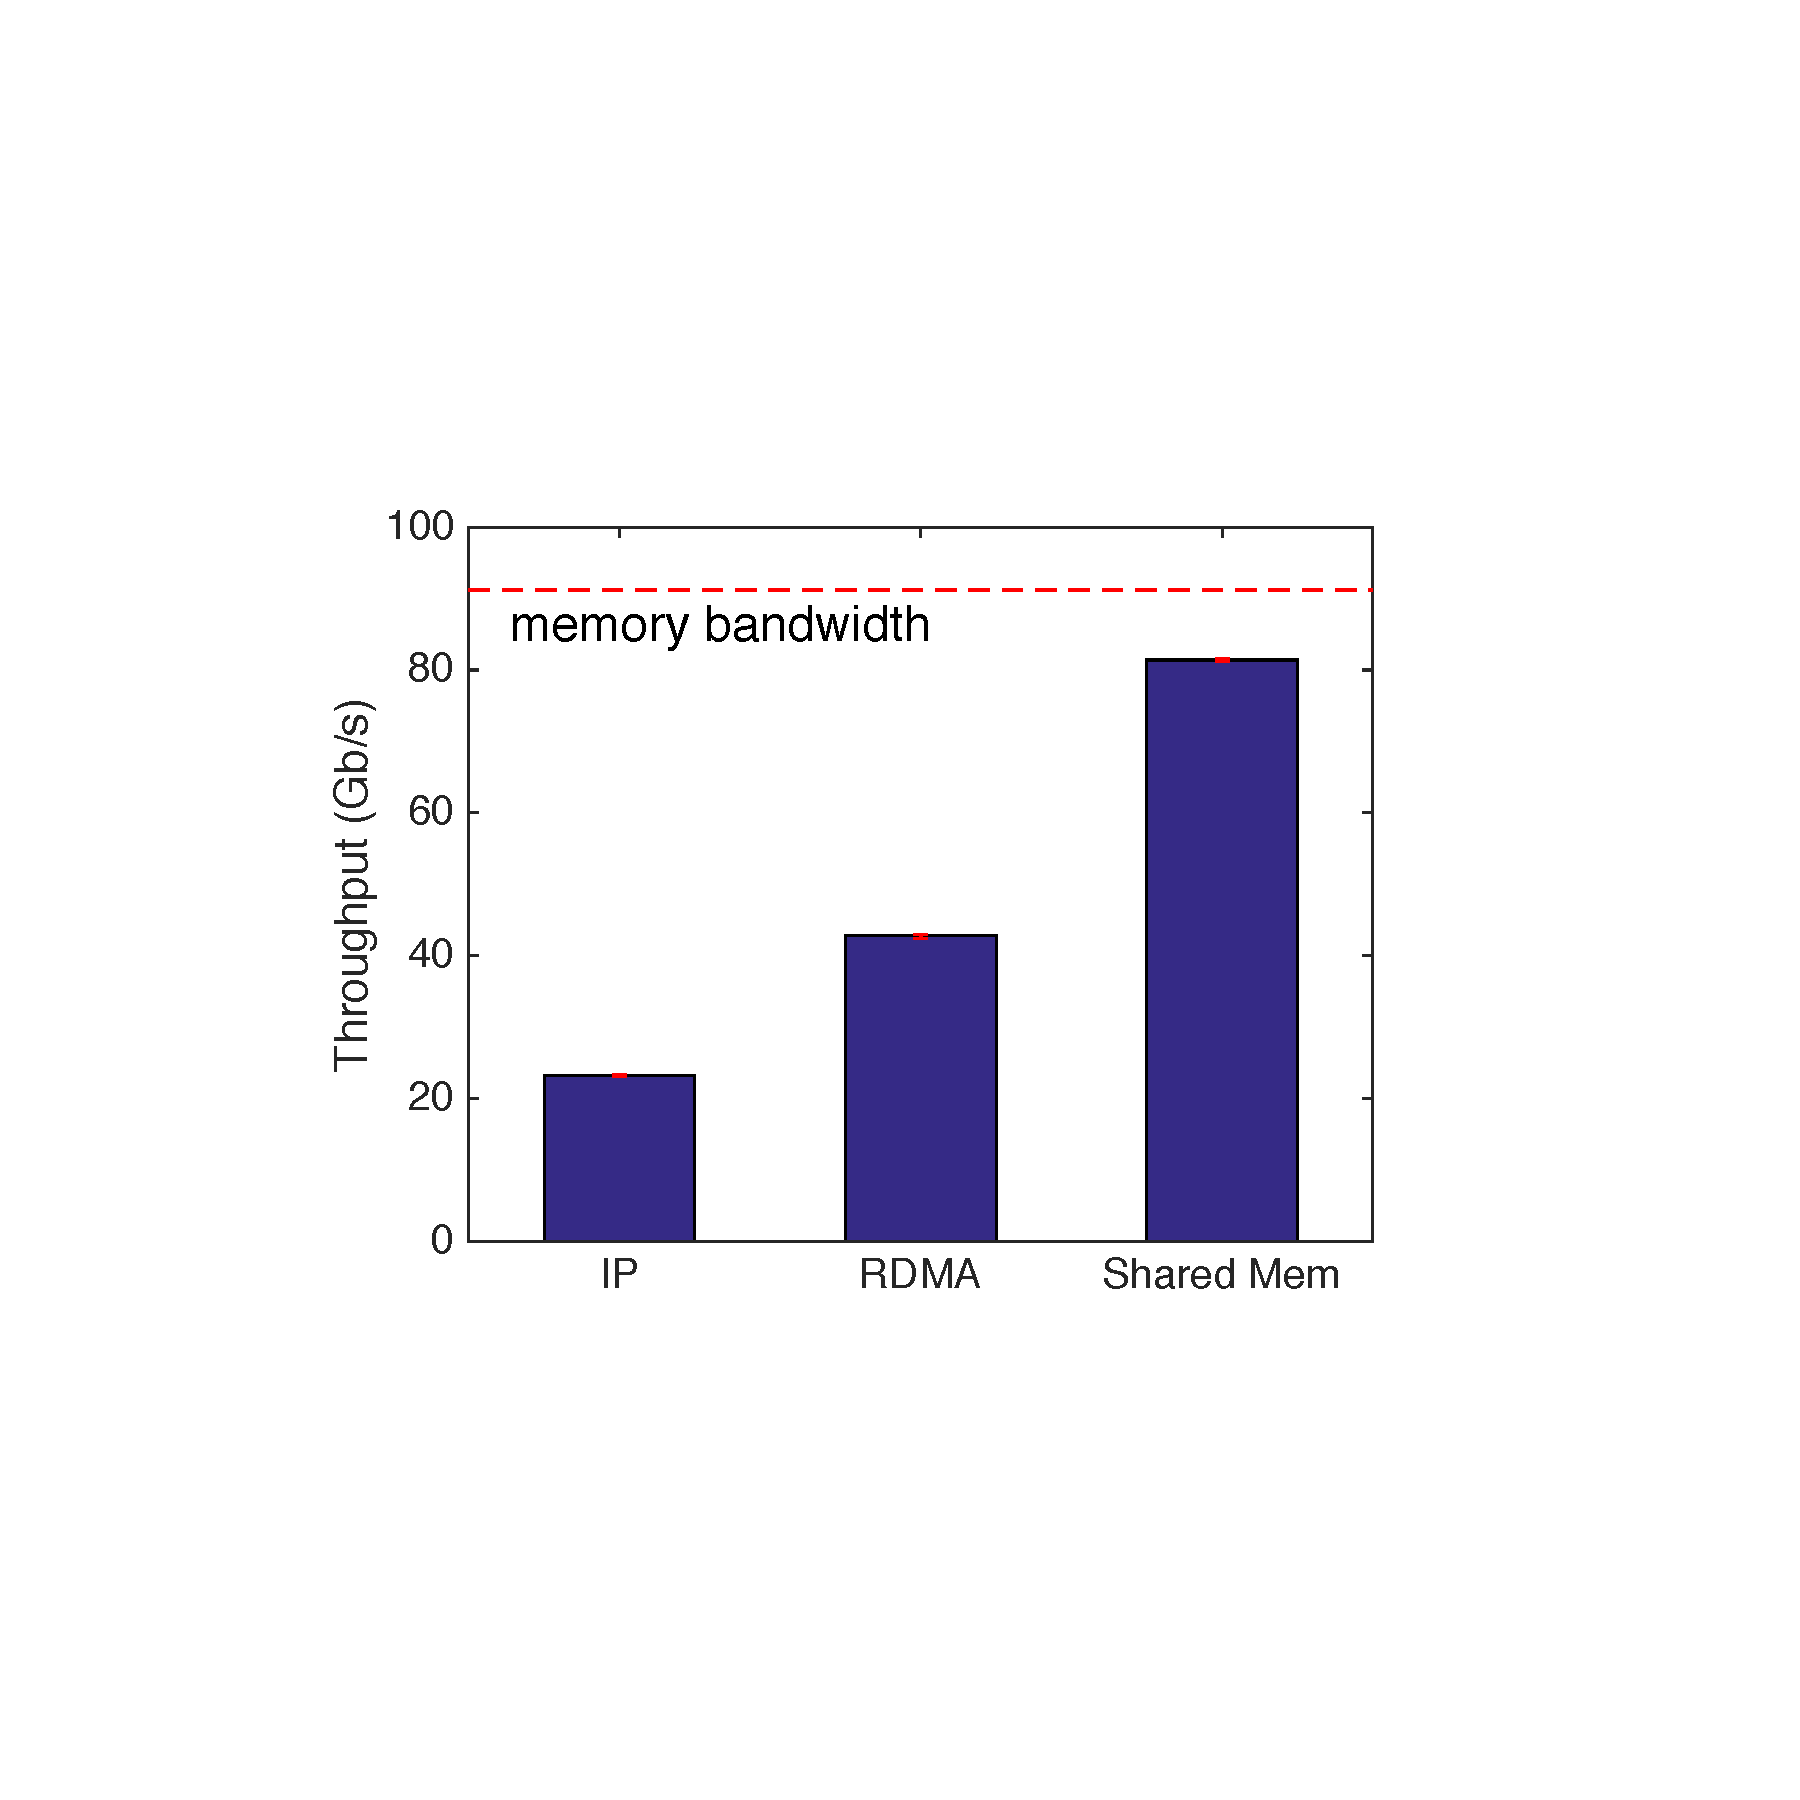
\includegraphics[width=0.32\textwidth]{figures/motivation/eval_baremetal_thr.pdf}      
     %\label{fig:eval_baremetal_thr}
     %\caption{} 
     \end{subfigure}      
     \begin{subfigure}[t]
     \centering 
     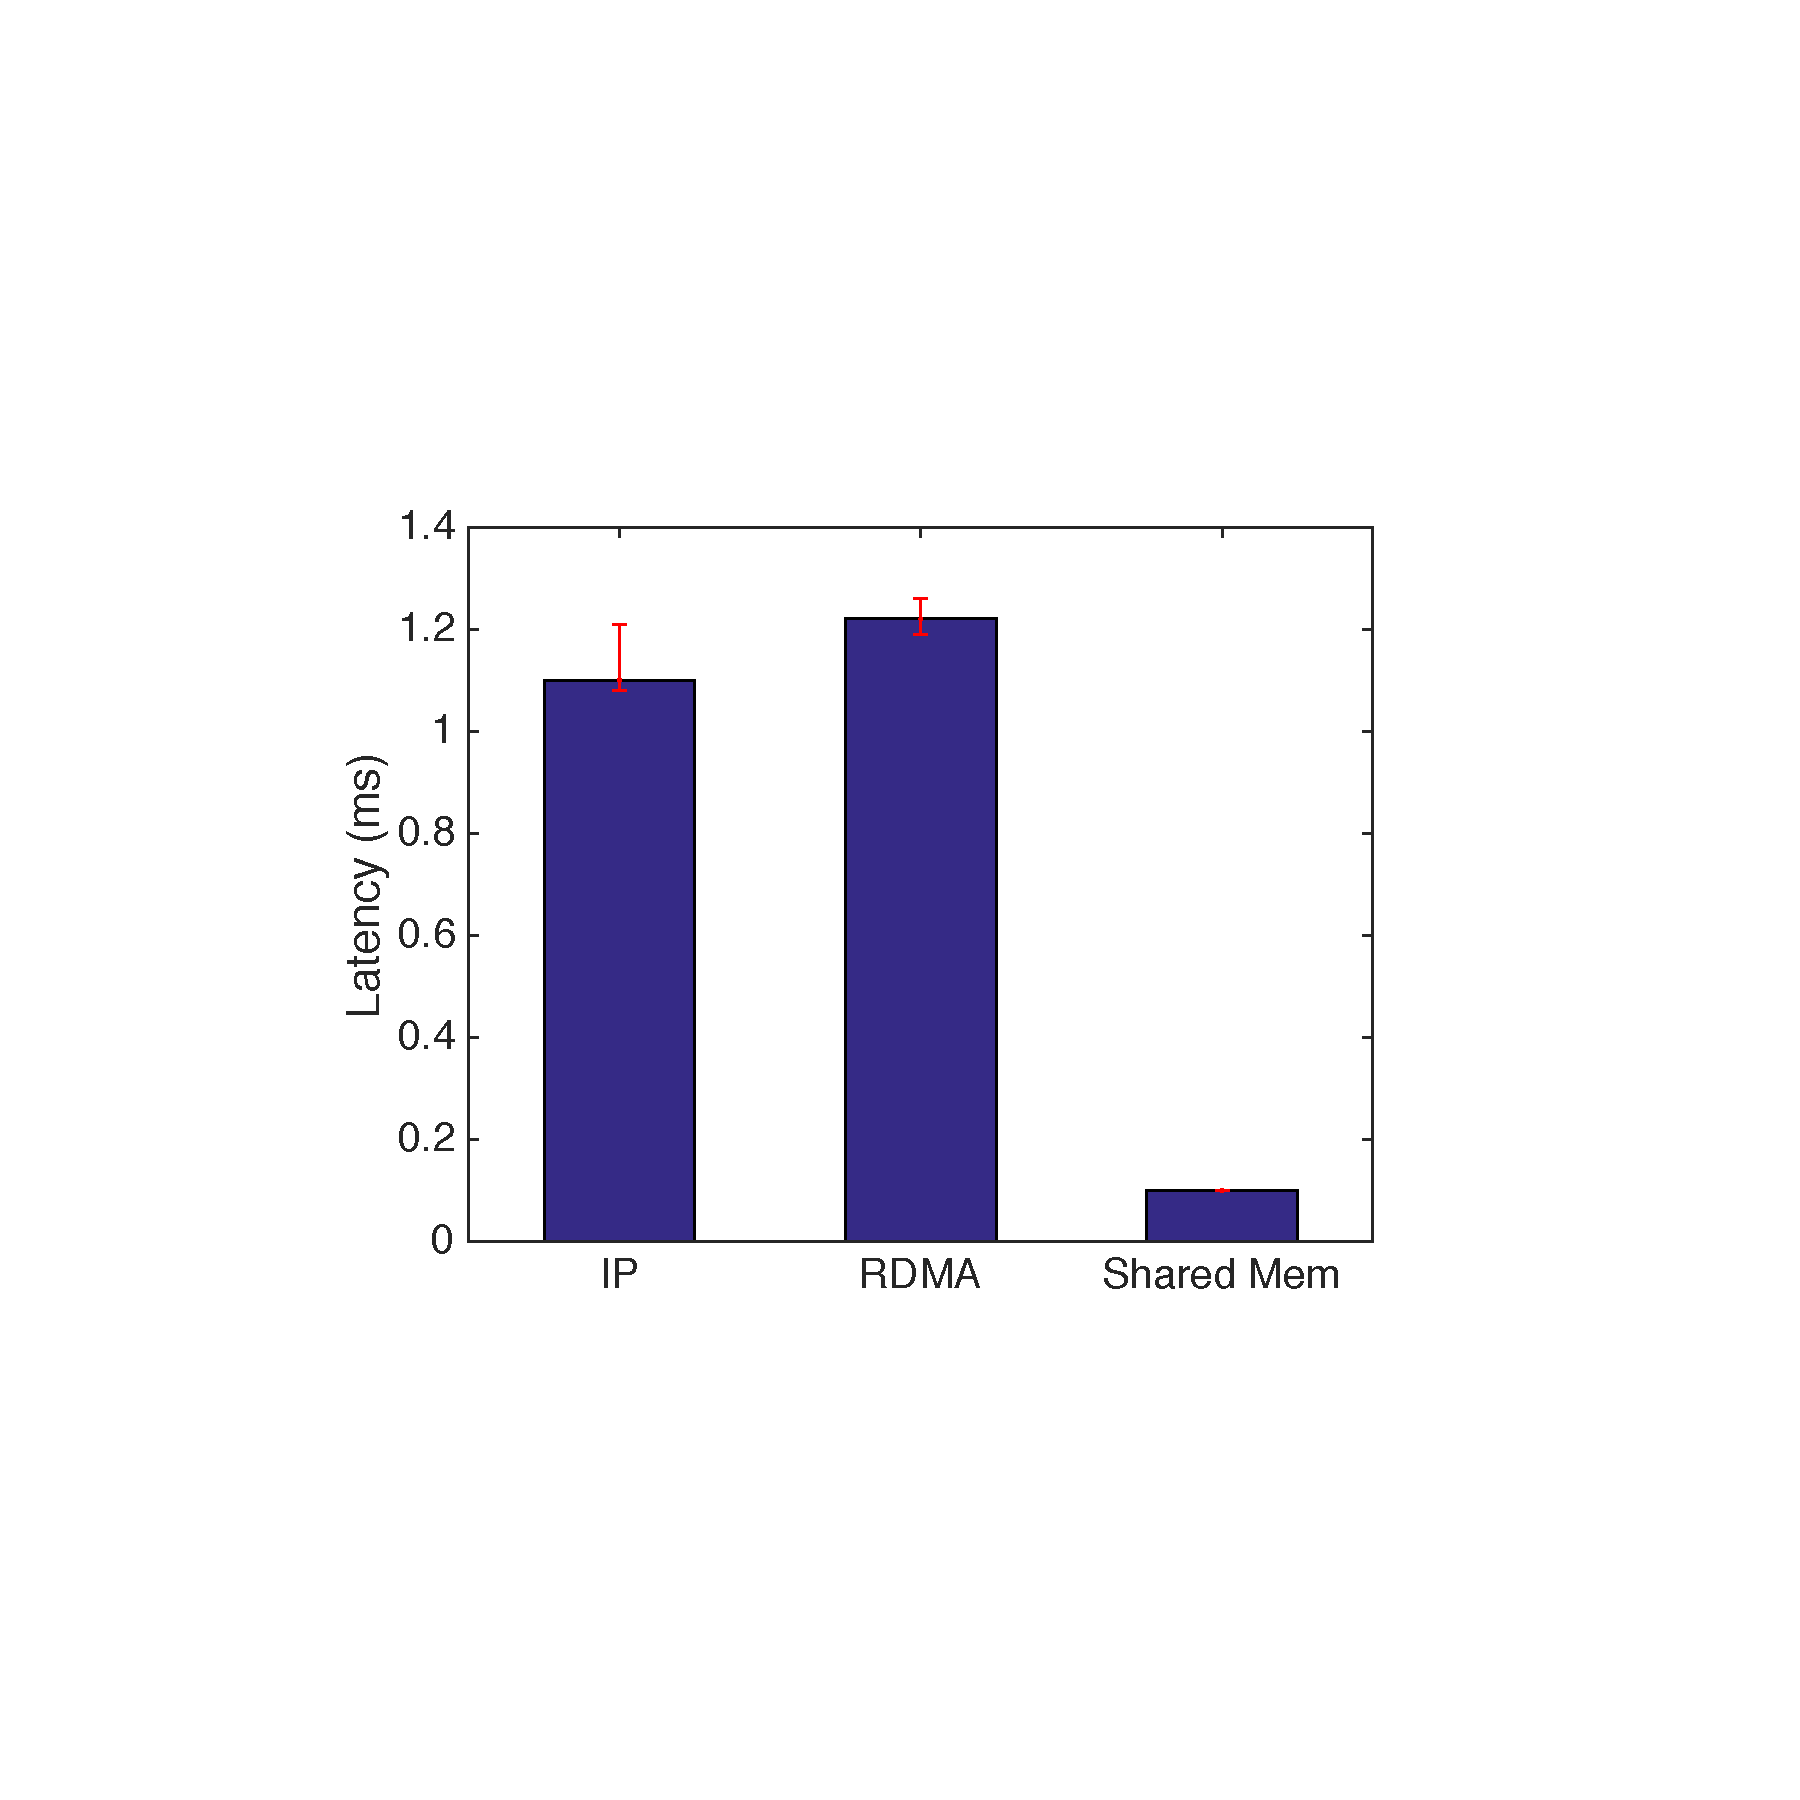
\includegraphics[width=0.32\textwidth]{figures/motivation/eval_baremetal_latency.pdf}      
     %\label{fig:eval_baremetal_latency}
     %\caption{} 
     \end{subfigure}      
     \begin{subfigure}[t]
     \centering 
     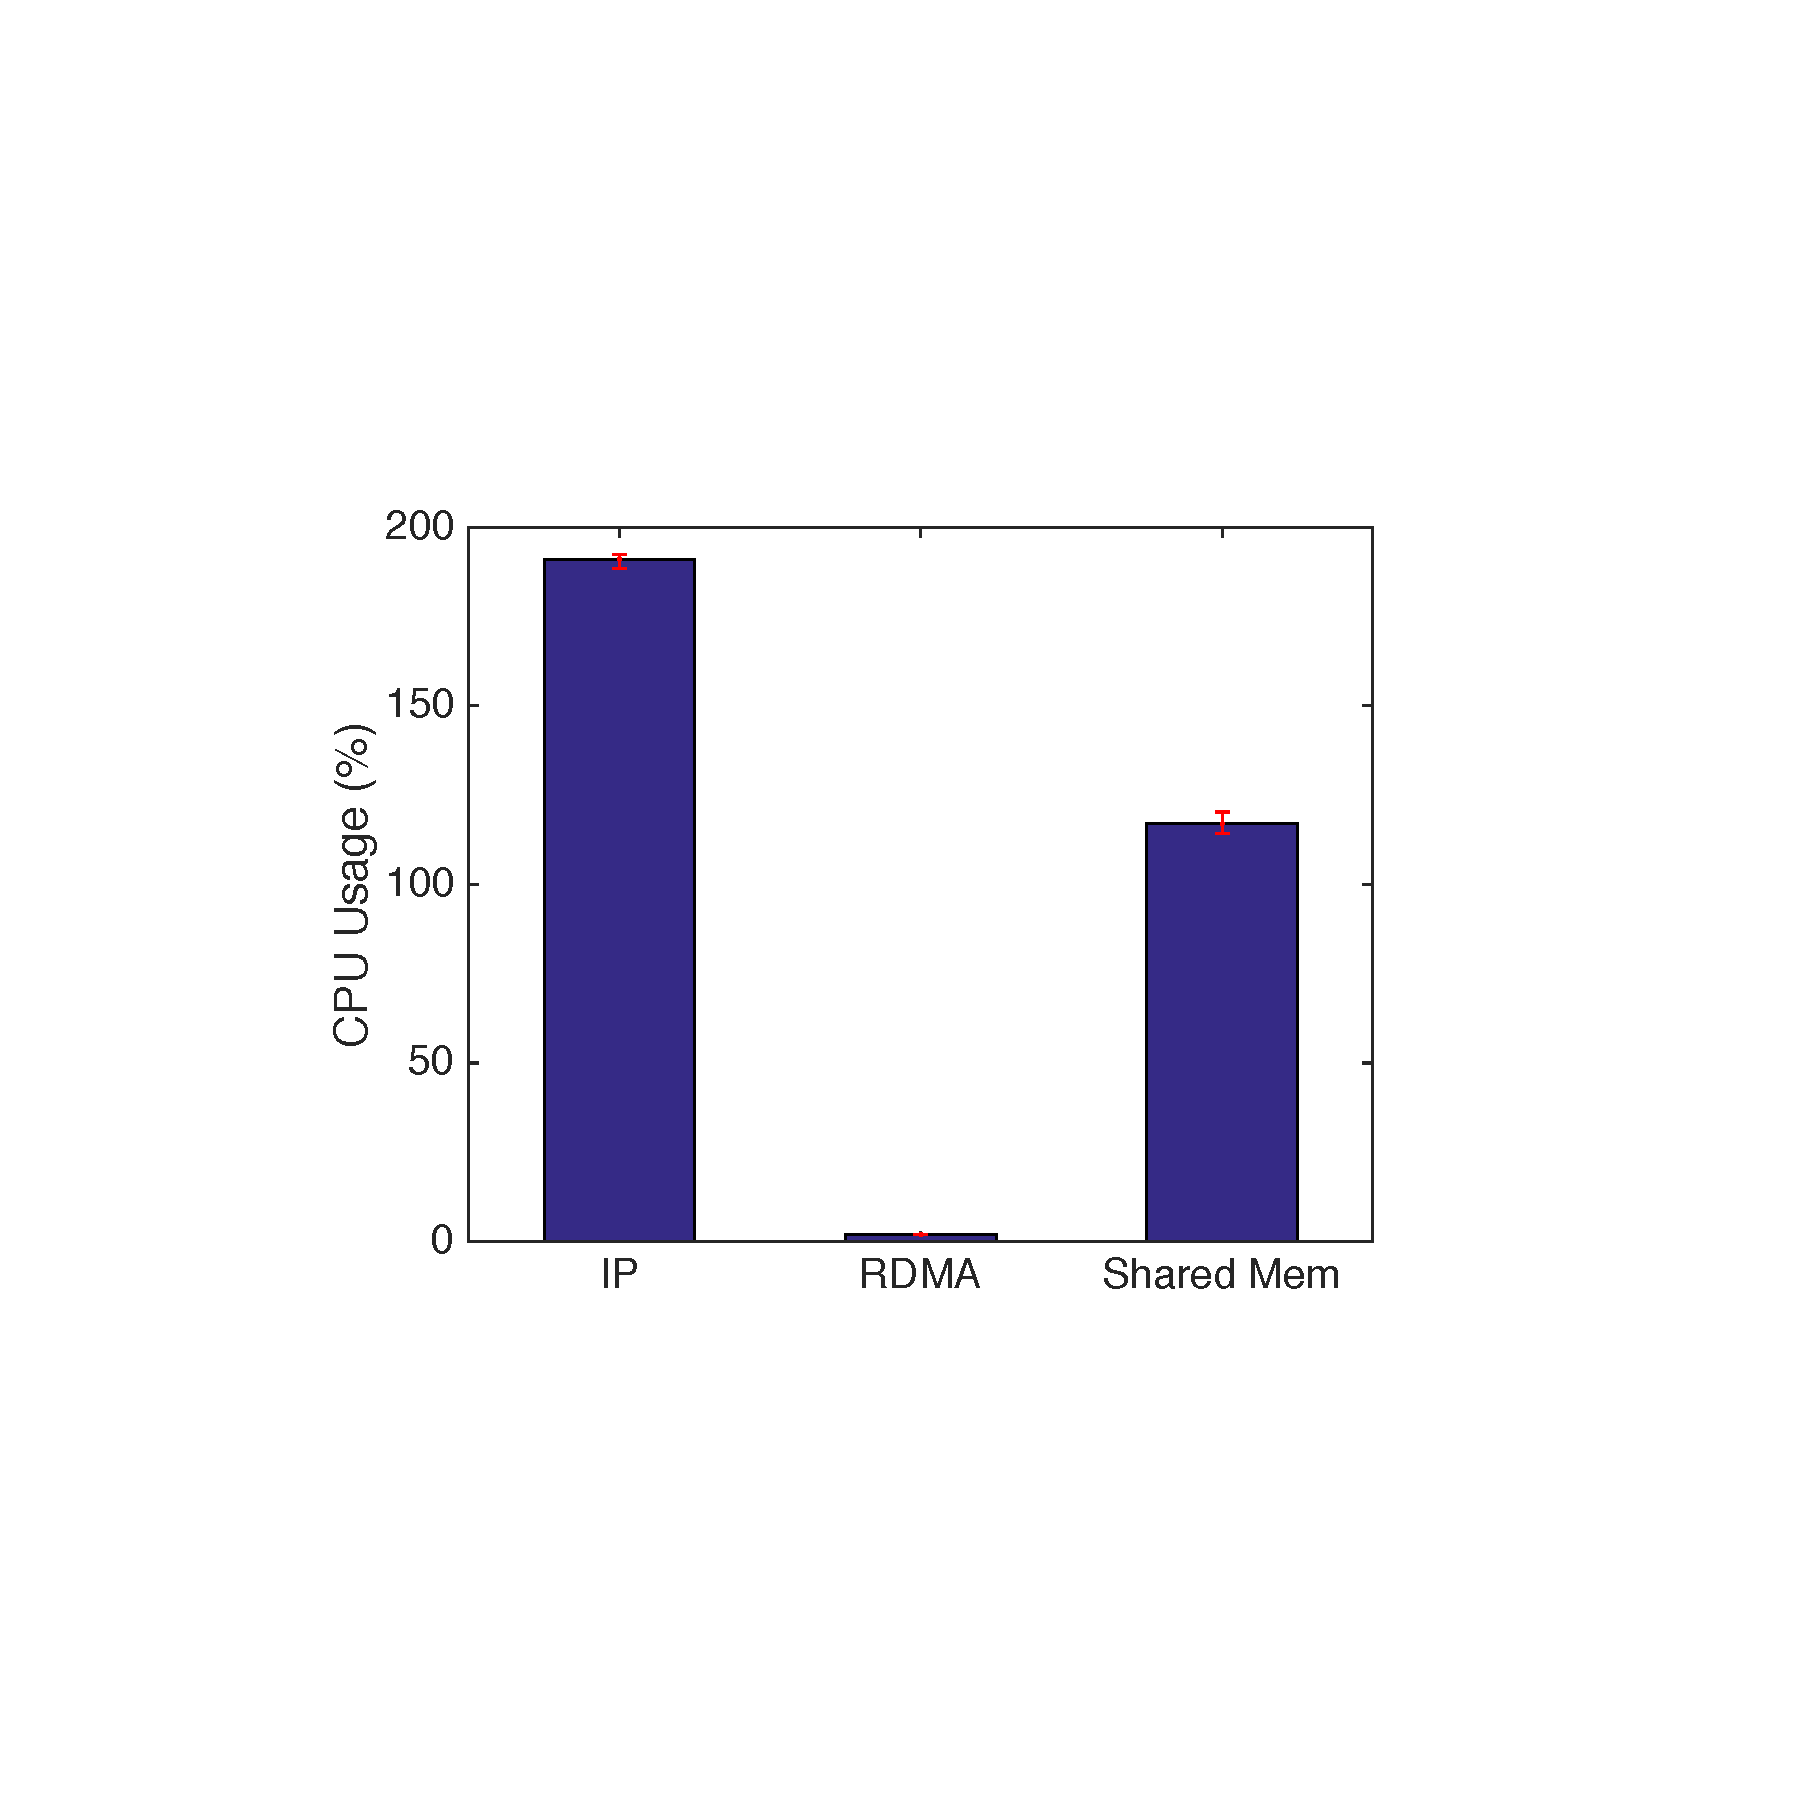
\includegraphics[width=0.32\textwidth]{figures/motivation/eval_baremetal_cpu.pdf}      
     %\label{fig:eval_baremetal_cpu}
     %\caption{} 
     \end{subfigure}           
     \label{fig:eval_baremetal_thr_latency_cpu}
     \caption{} 
\end{figure*} 

\begin{itemize}
  \item Communication via IP stack only achieves 27Gb/s throughput, 1 ms latency but uses near to 200\% of cpu.
  \item RDMA only improves the throughput to 40Gb/s for containers on the same machine, the latency is still 1ms, though it has a low cpu usage.
  \item Shared memory can achieve near-to-memory-bandwidth throughput, lowest latency, but still burns some cpu. 
\end{itemize}


\subsubsection{Host-mode vs. bridge mode}

\begin{figure}[!ht]
     \centering 
     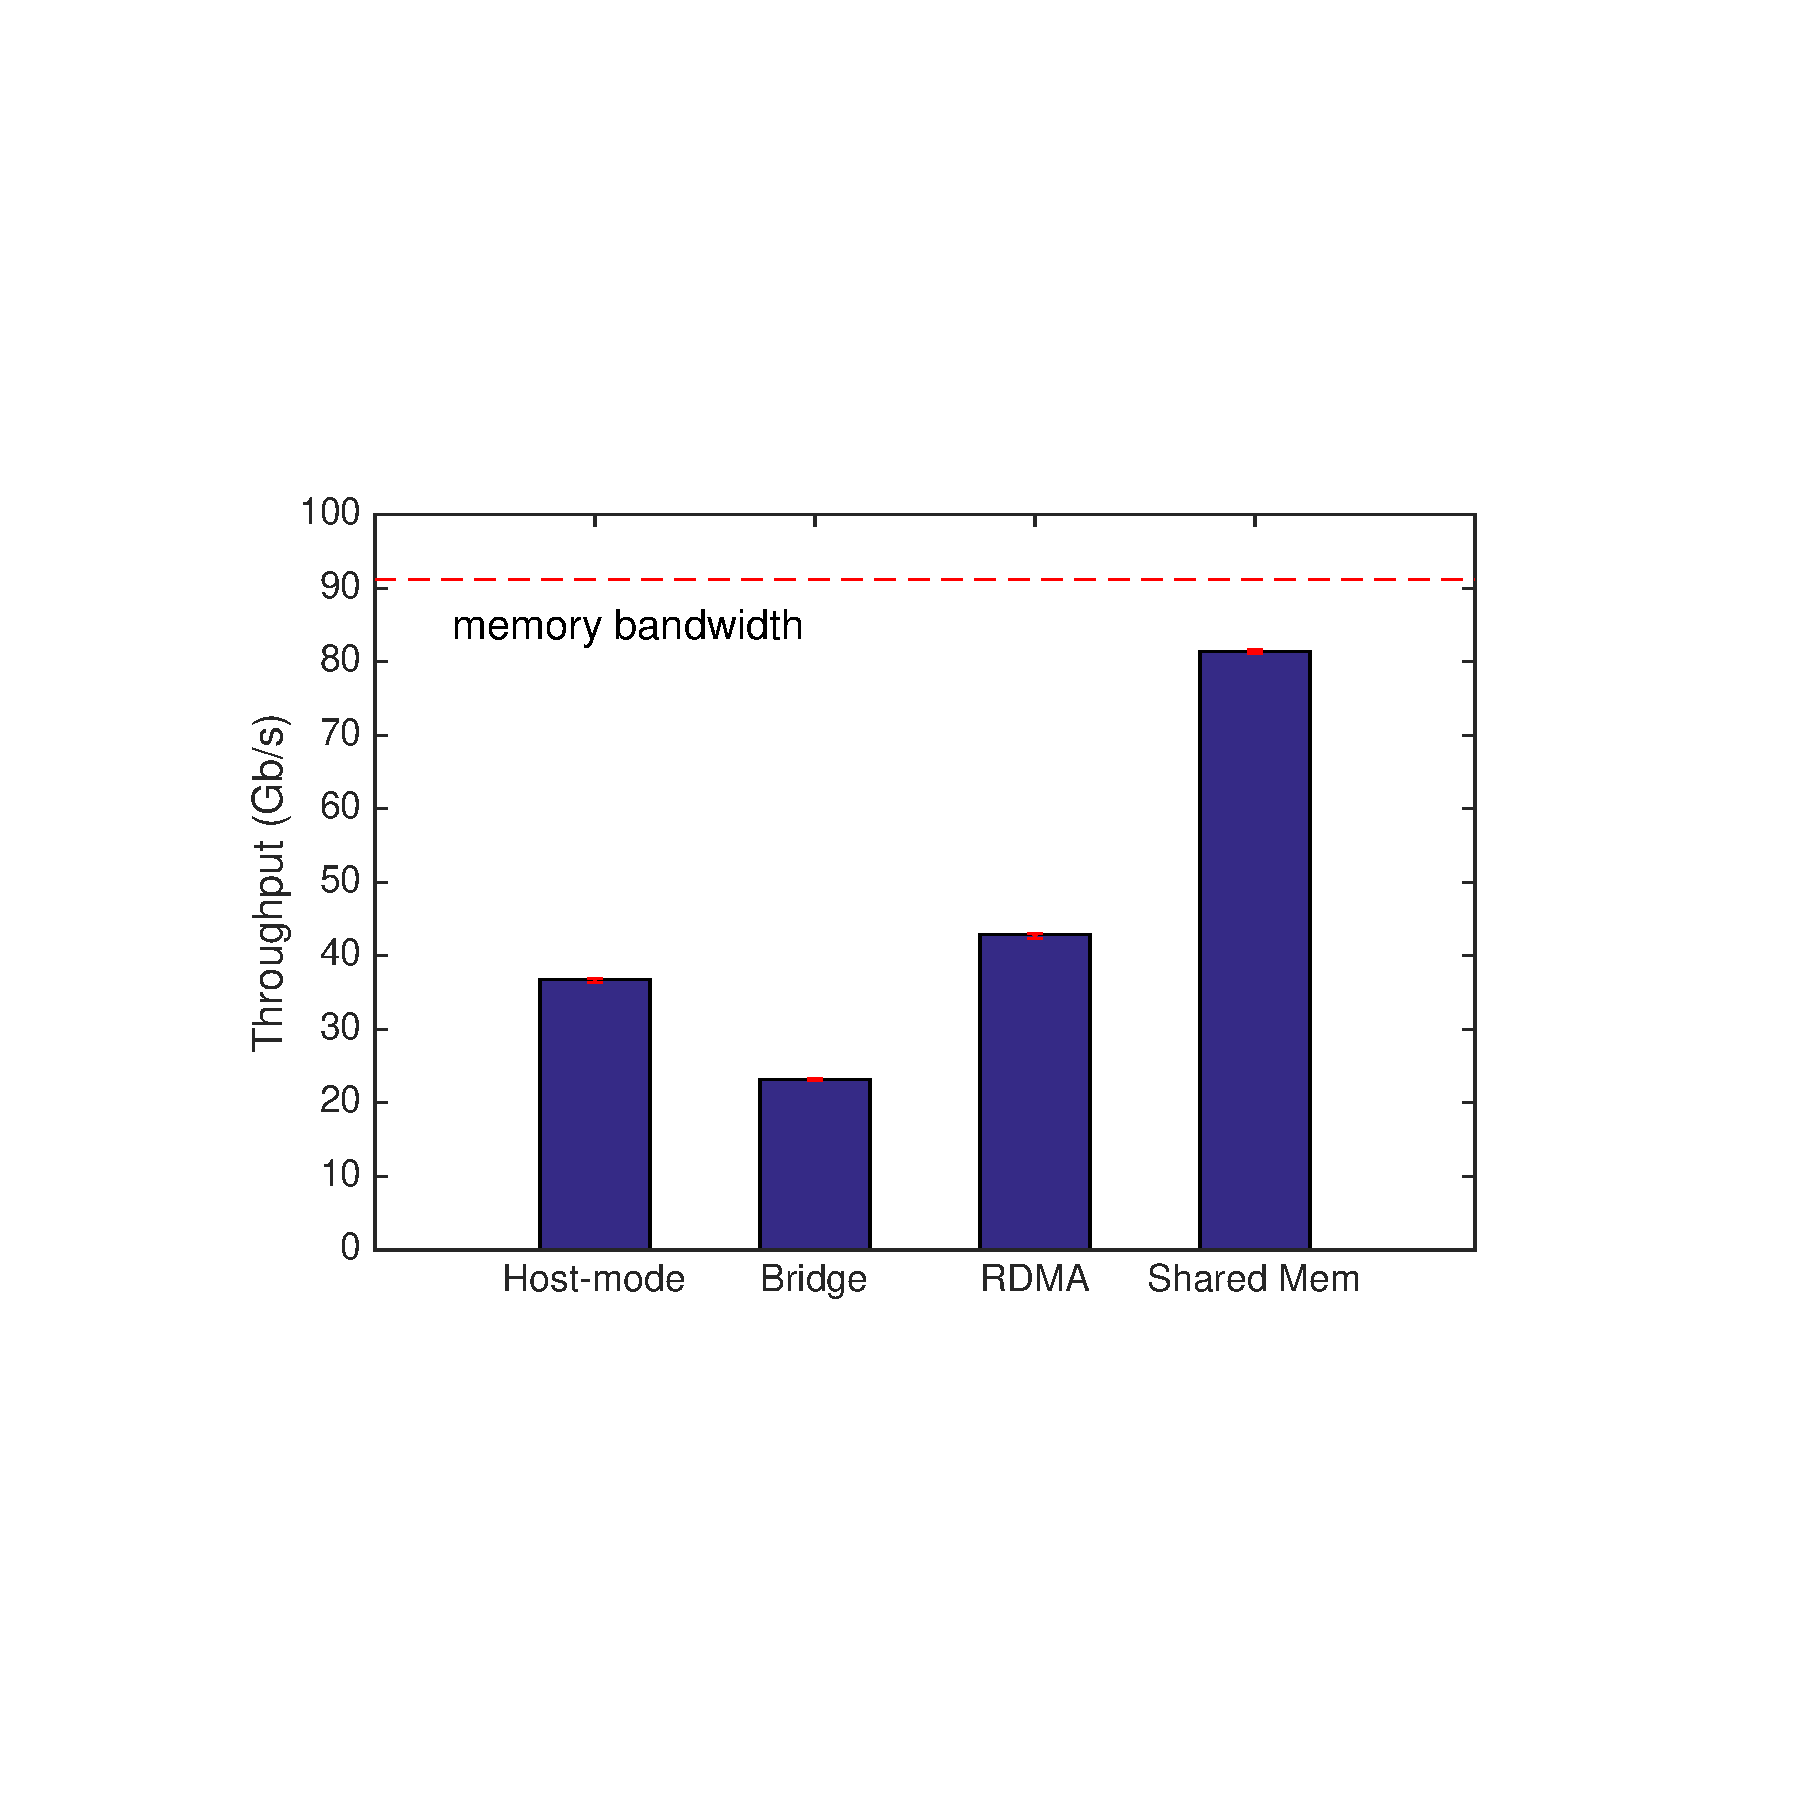
\includegraphics[width=3.35in]{figures/motivation/eval_bw_host_bridge.pdf} 
     \label{fig:eval_bw_host_bridge}
     \caption{ Host-mode vs. bridge mode vs. RDMA vs. shared memory.} 
\end{figure} 

\begin{itemize}
  \item Host-mode provides a better performance of 38 Gb/s. 
\end{itemize}

\subsection{Intra-host Network Performance}

\para{Throughput}

Three points: (1) TCP throughput is limited; (2) the bottleneck is CPU rather than memory bus for TCP/IP; (3) the bottleneck is NIC CPU for RDMA. (4) For intra-host cases, shared memory has the best performance.

Figure 1: throughput of single src-dst pair. Bar figure: x-axis: TCP/IP, RDMA and shared memory; y-axis: throughput;

Figure 2(a): throughput of multiple src-dst pair. Line figure: x-axis: number of pairs,; y-axis: throughput; Four lines: TCP/IP, RDMA, shared memory and memory bus.

Figure 2(b): CPU utilization. Line figure: x-axis: number of pairs,; y-axis: CPU utilization; Three lines: TCP/IP, RDMA, shared memory.

Figure 2(c): NIC CPU utilization. Line figure: x-axis: number of pairs,; y-axis: NIC CPU utilization; Three lines: TCP/IP, RDMA, shared memory.

\begin{figure}[!ht]
     \centering 
     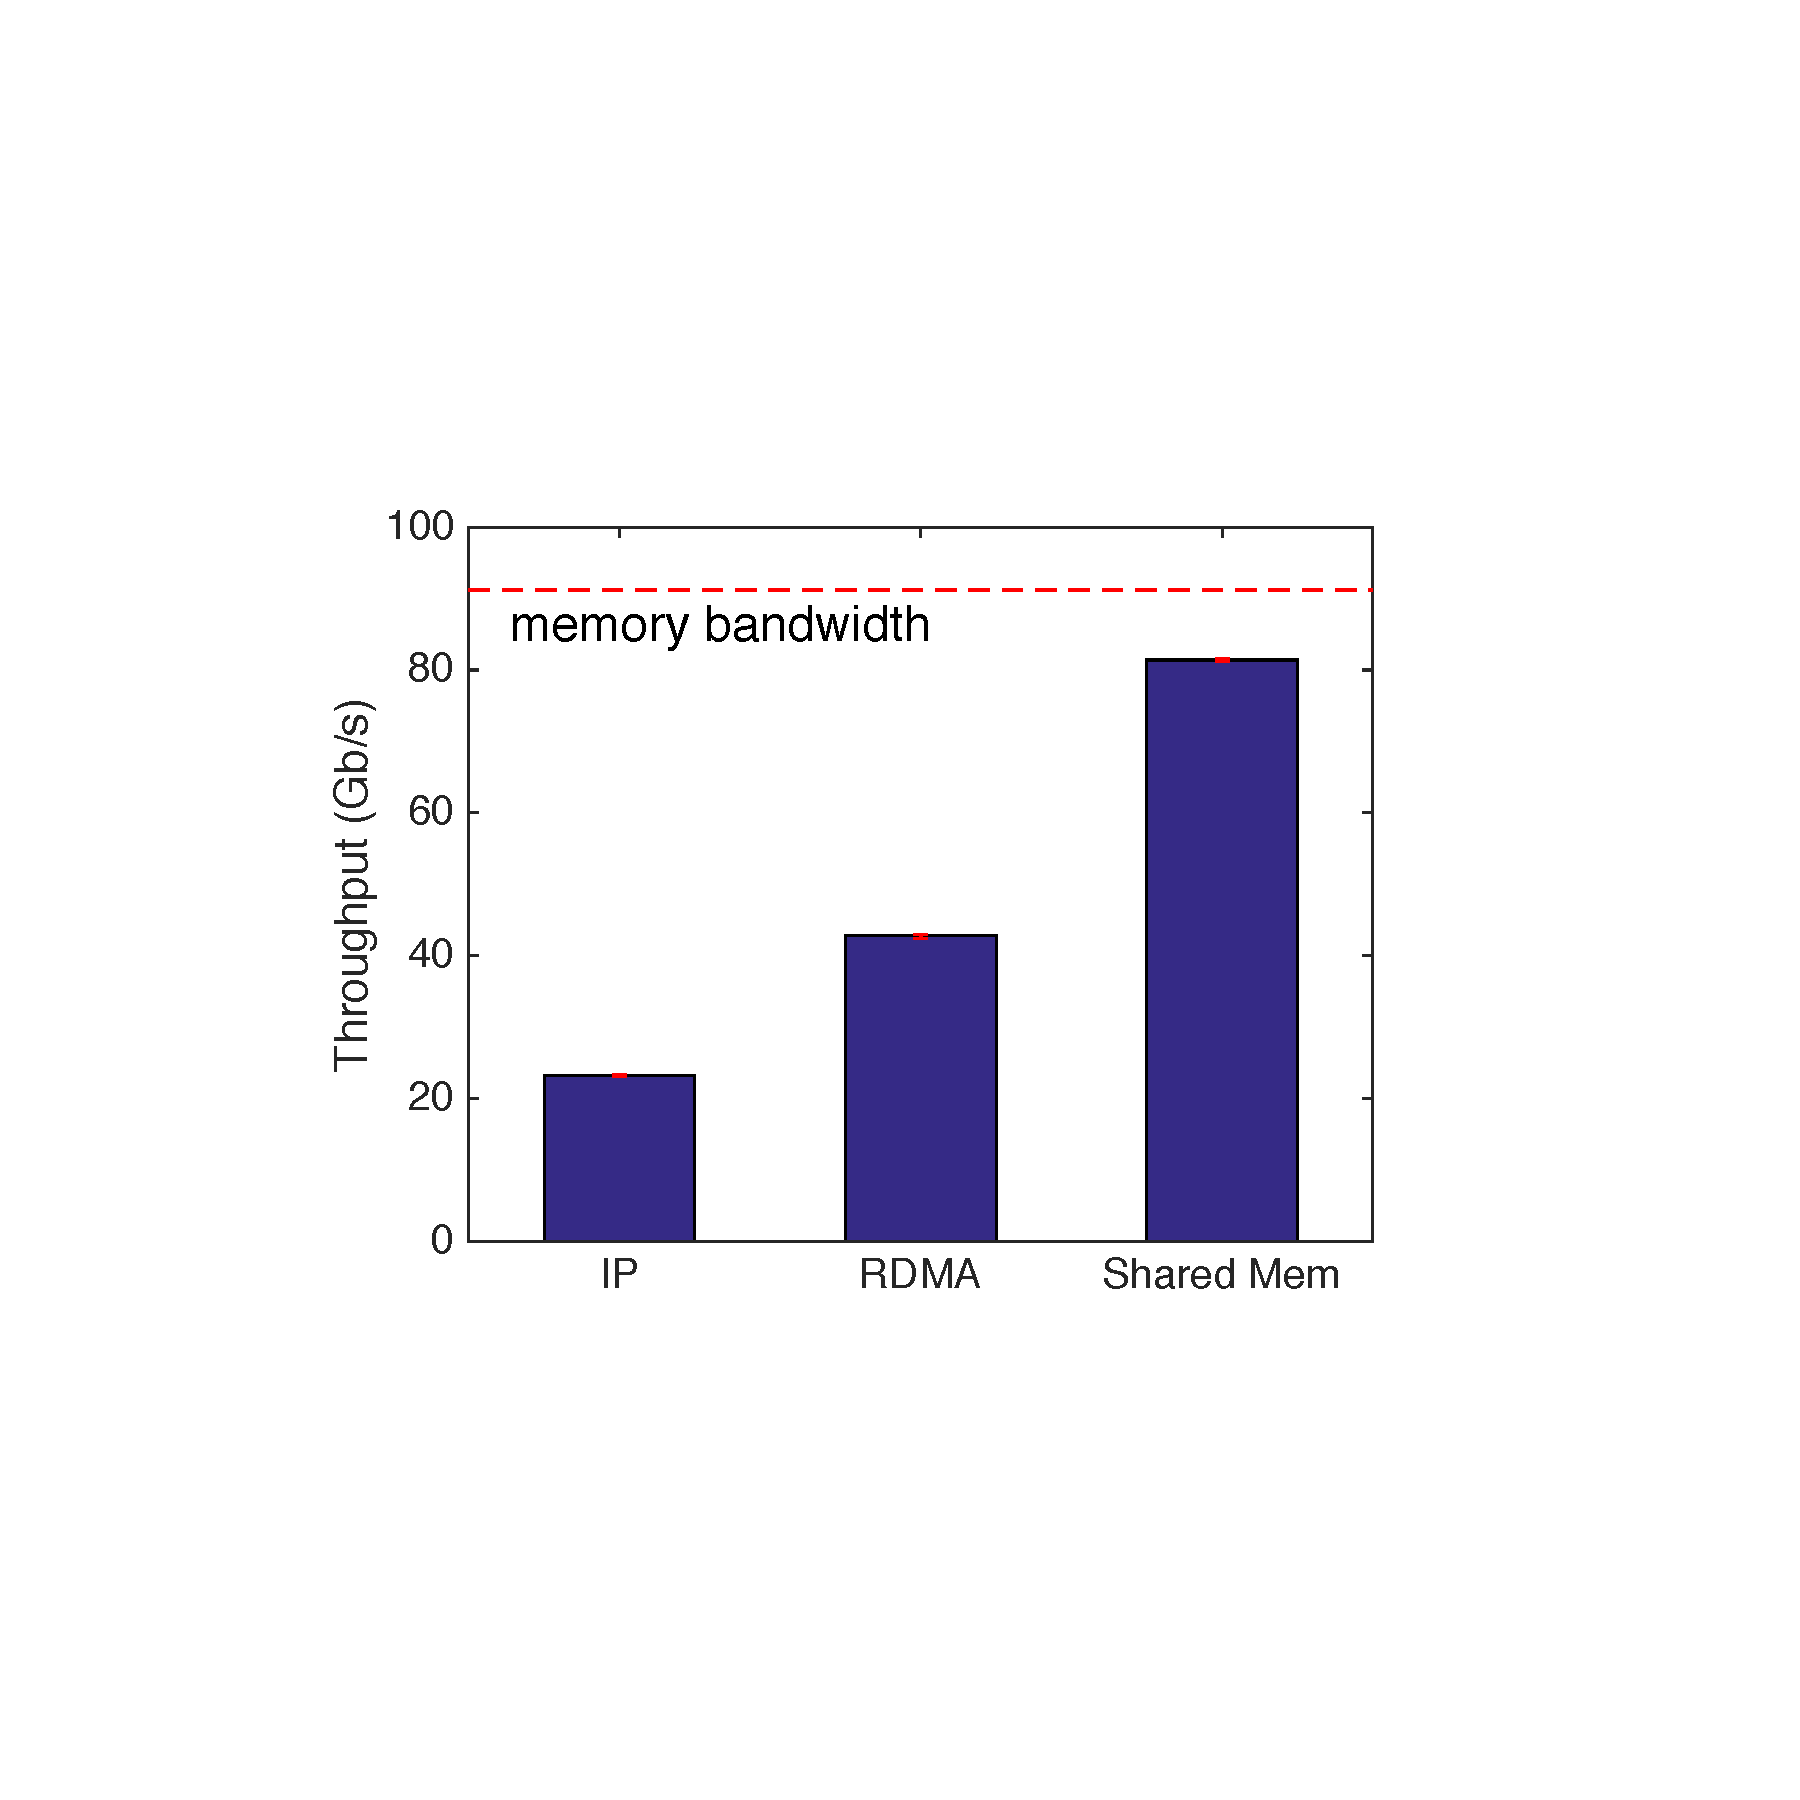
\includegraphics[width=3.35in]{figures/motivation/eval_baremetal_thr.pdf} 
     \caption{\label{fig:eval_baremetal_thr} The throughput of a pair of containers on the same bare metal communicating via IP stack, RDMA and shared memory. Communication via shared memory is close to the memory bandwidth.} 
\end{figure} 

\para{Latency}
Two points: (1) going through OS stack is increasing network latency; (2) The bottleneck is on system calls.

Figure 3: The stacked bar chart showing the total latency of TCP/IP, RDMA, shared memory and their components.

\begin{figure}[!ht]
     \centering 
     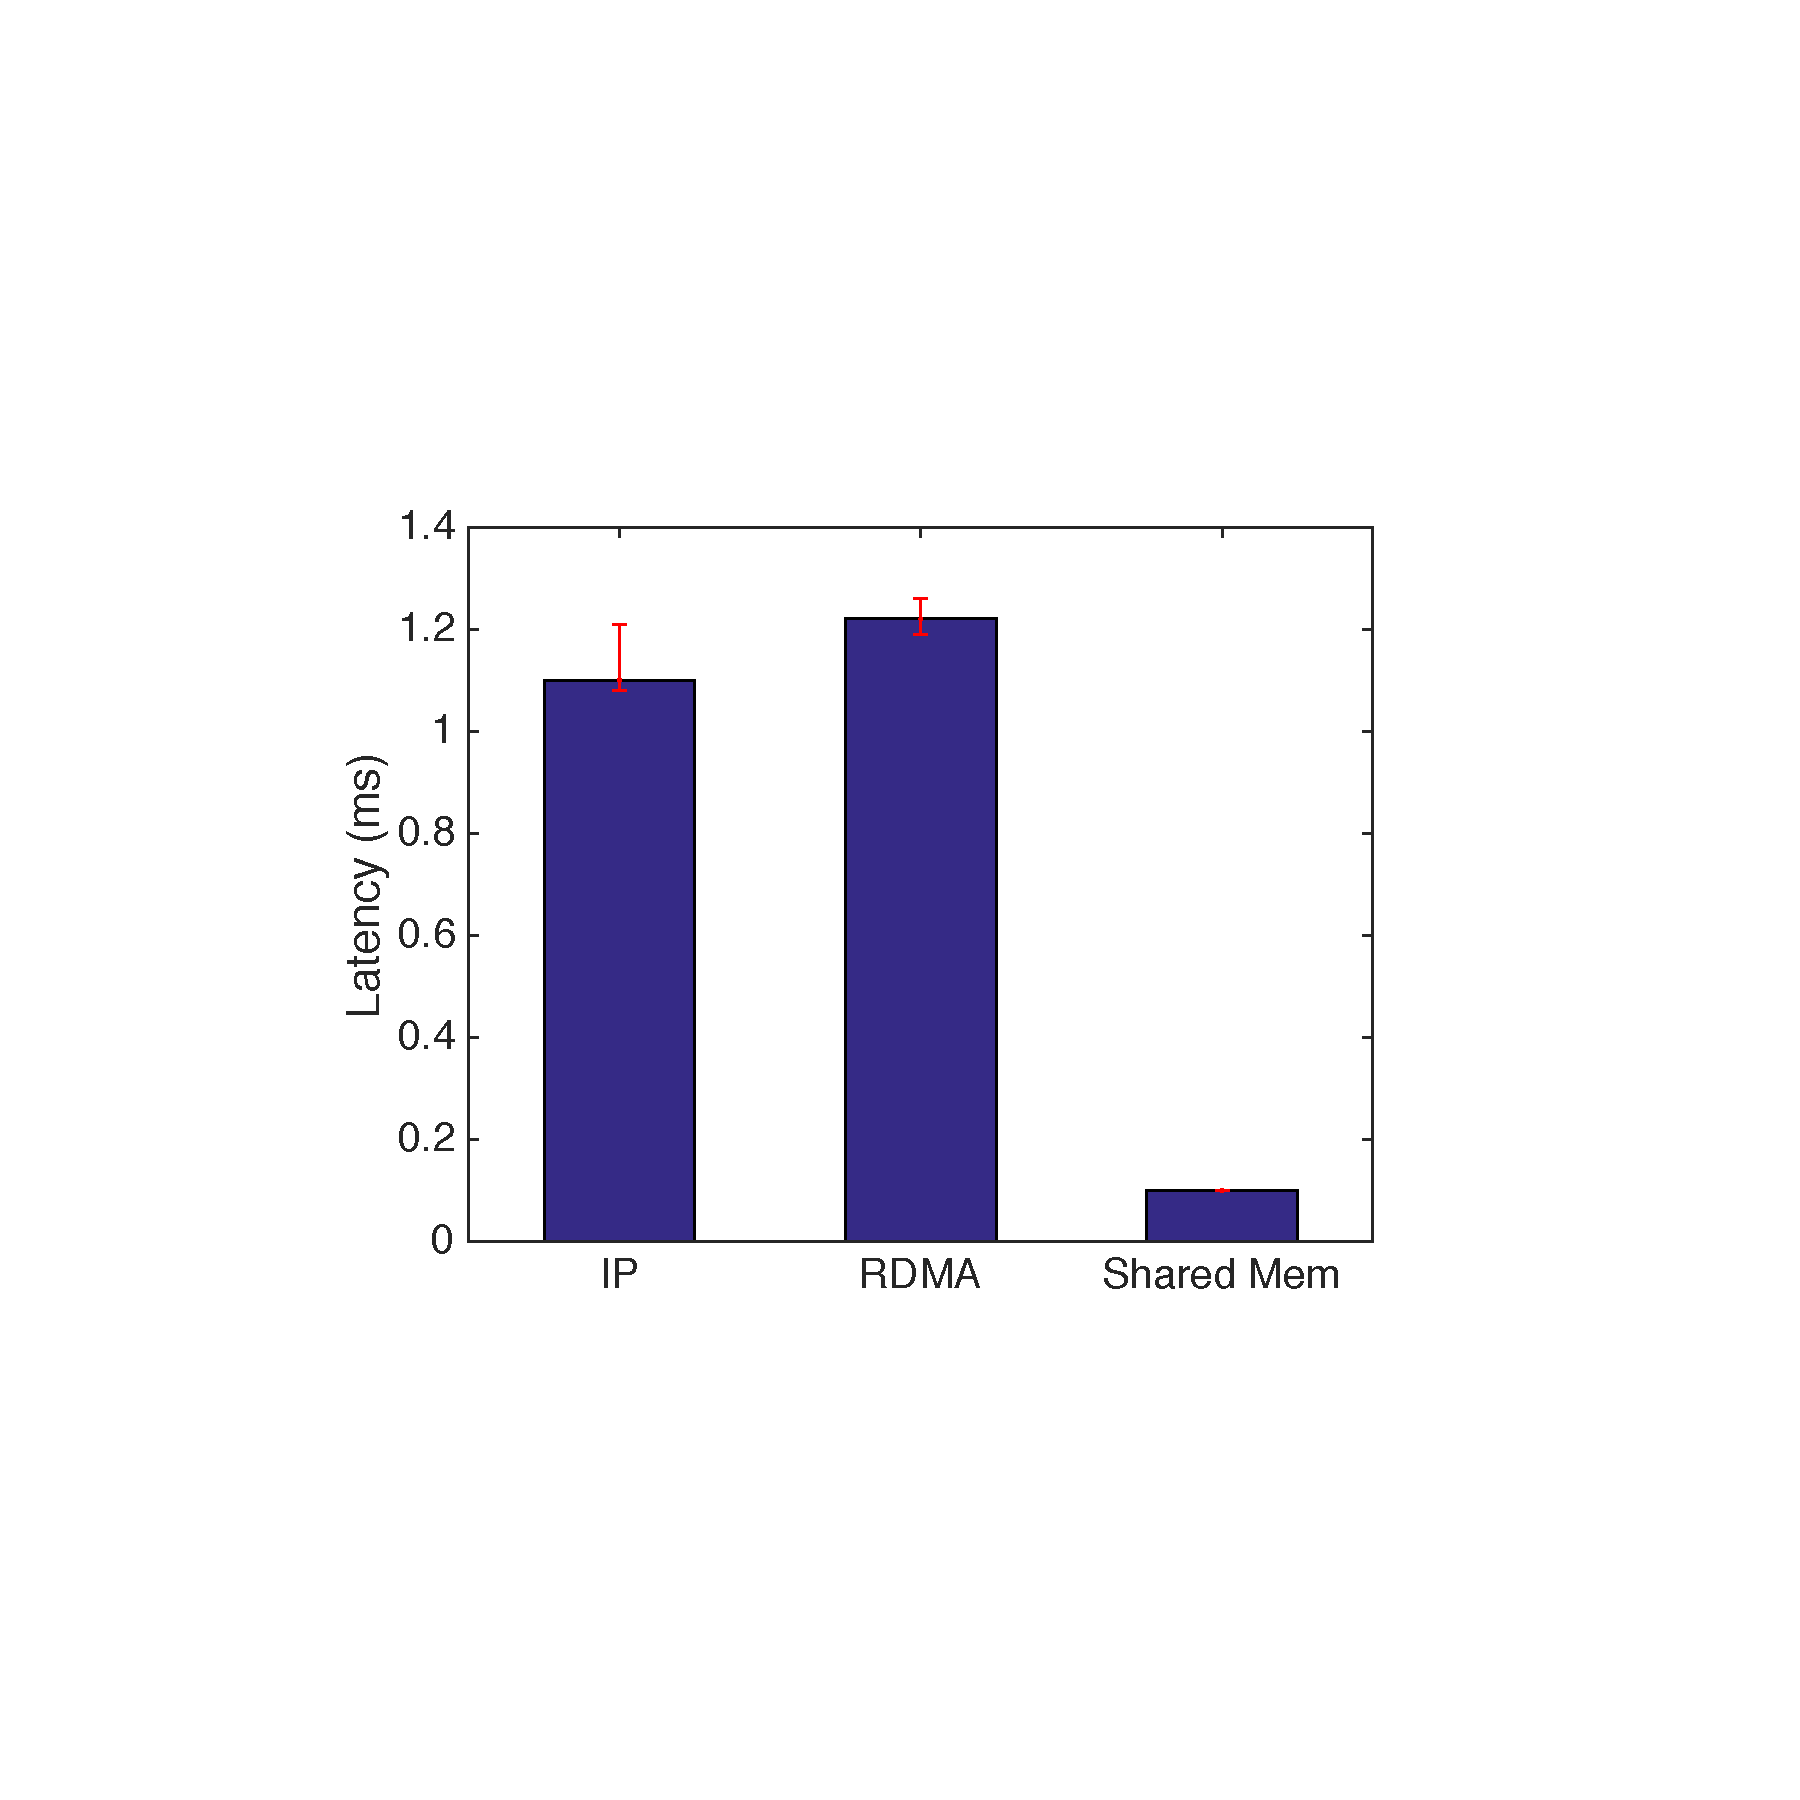
\includegraphics[width=3.35in]{figures/motivation/eval_baremetal_latency.pdf} 
     \caption{\label{fig:eval_baremetal_latency} The latency of a pair of containers on the same bare metal communicating via IP stack, RDMA and shared memory. Shared memory achieves the lowest latency.} 
\end{figure} 

\para{CPU Usage}

\begin{figure}[!ht]
     \centering 
     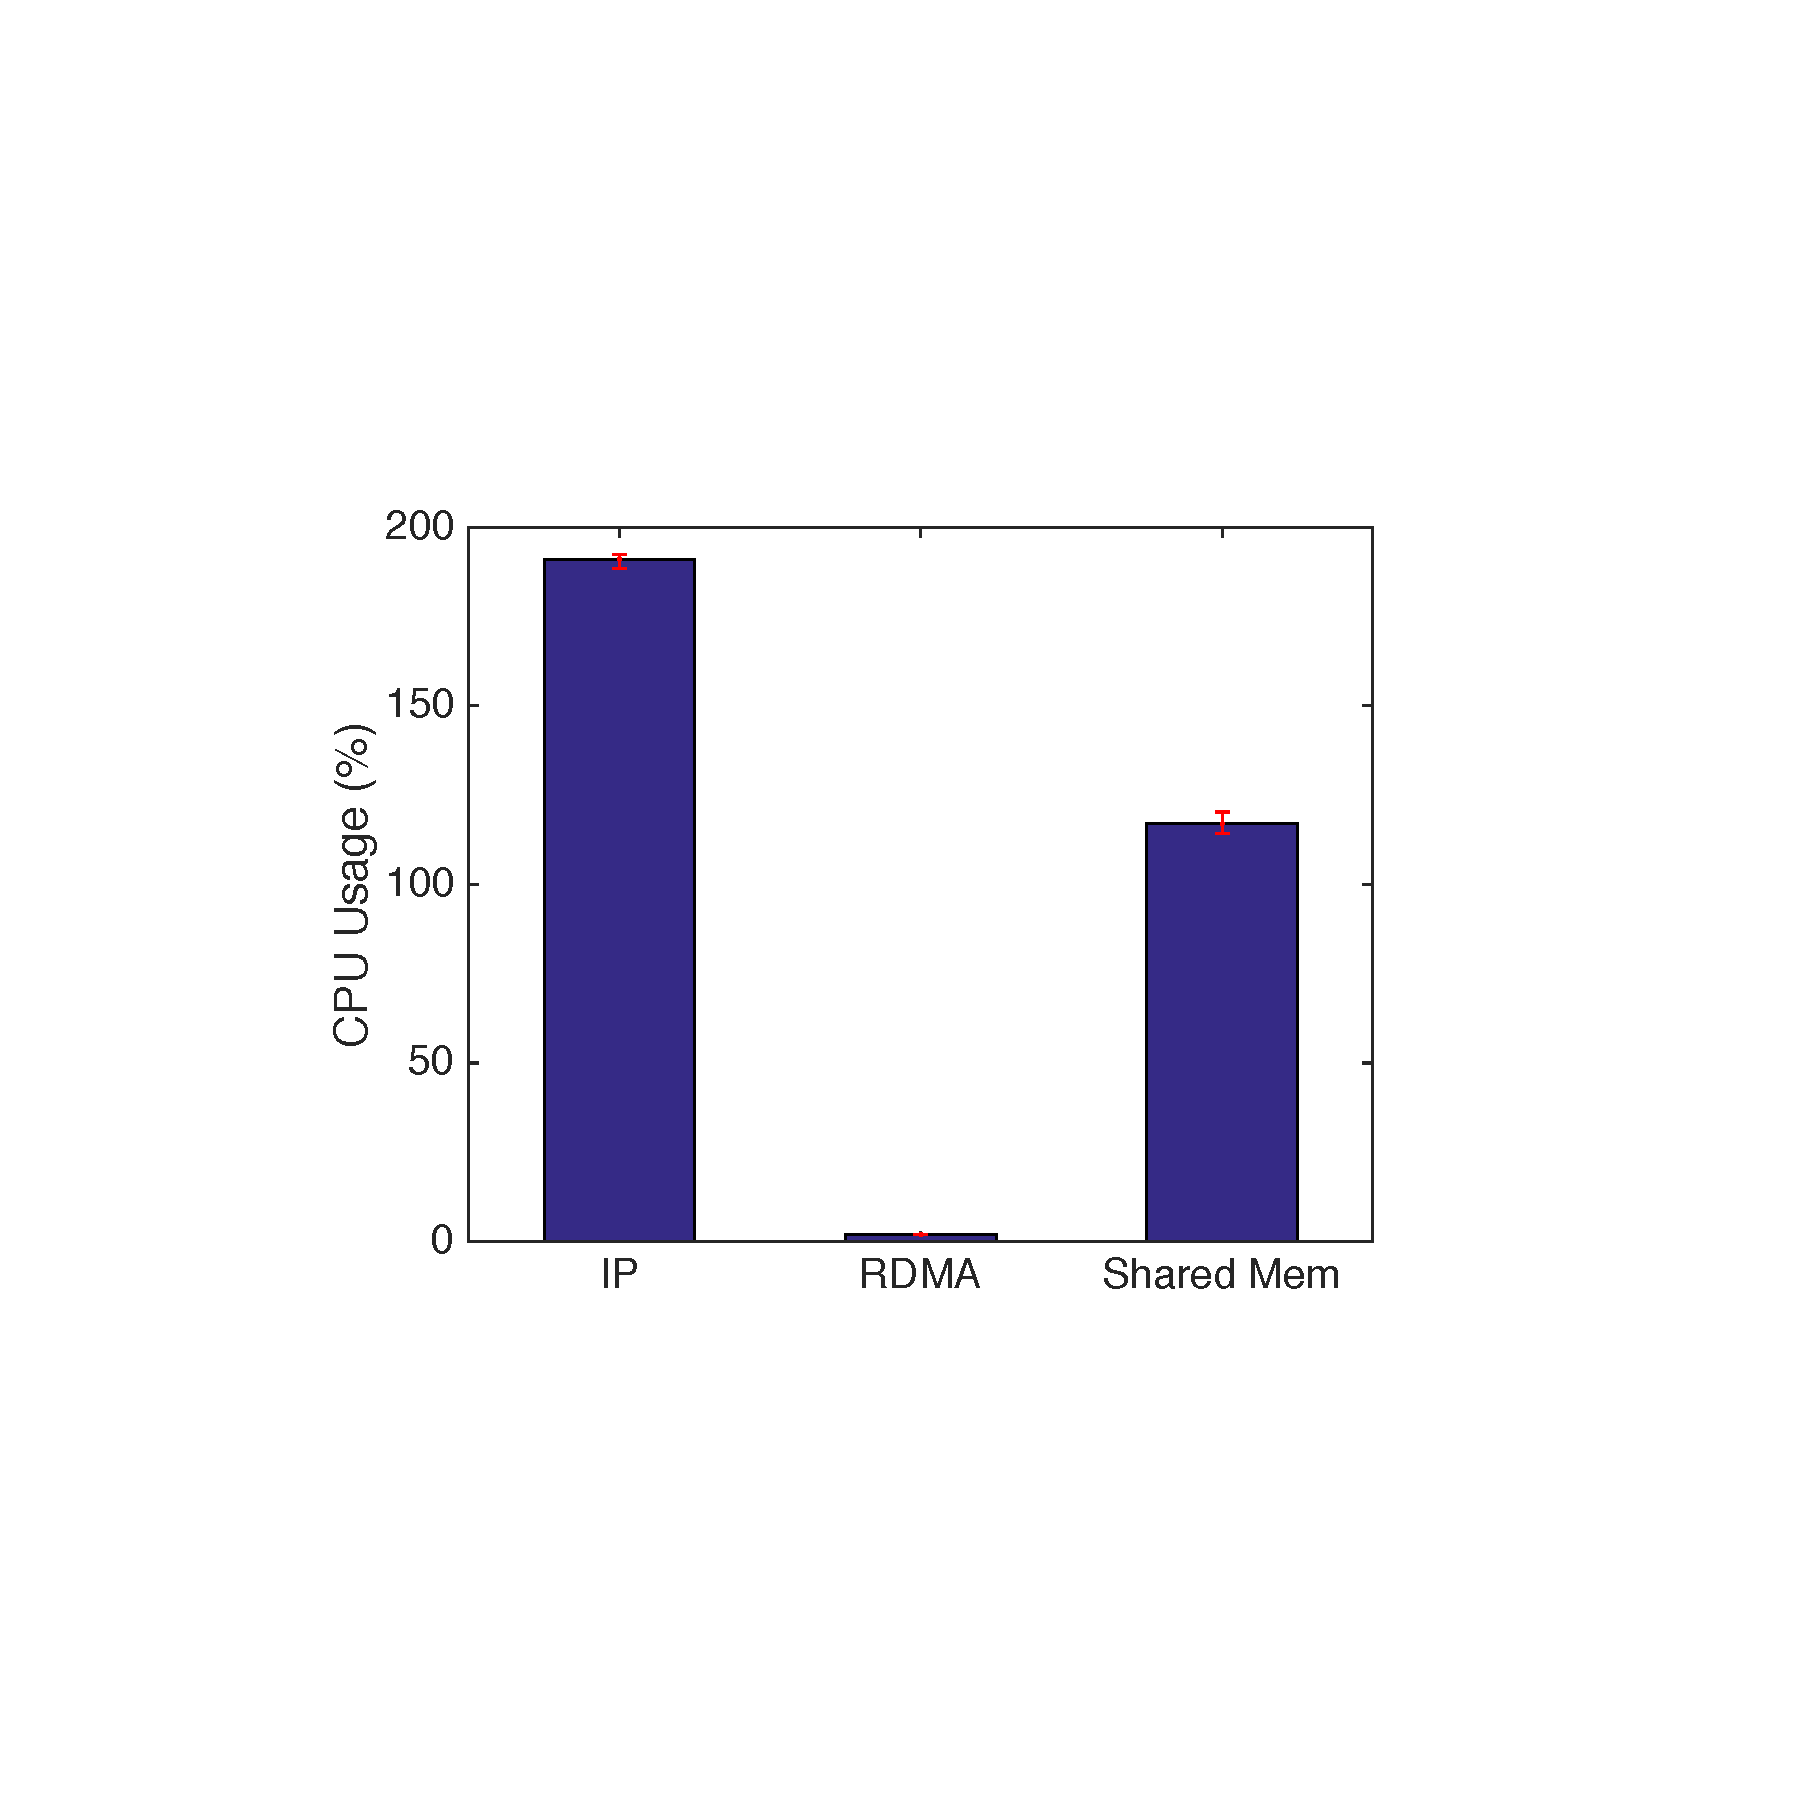
\includegraphics[width=3.35in]{figures/motivation/eval_baremetal_cpu.pdf} 
     \caption{\label{fig:eval_baremetal_cpu} The cpu usage of a pair of containers on the same bare metal communicating via IP stack, RDMA and shared memory. Communication via IP stack almost saturates 2 cpu cores.} 
\end{figure} 

% comment 
\fi